\PassOptionsToPackage{unicode=true}{hyperref} % options for packages loaded elsewhere
\PassOptionsToPackage{hyphens}{url}
%
\documentclass[english,man,floatsintext]{apa6}
\usepackage{lmodern}
\usepackage{amssymb,amsmath}
\usepackage{ifxetex,ifluatex}
\usepackage{fixltx2e} % provides \textsubscript
\ifnum 0\ifxetex 1\fi\ifluatex 1\fi=0 % if pdftex
  \usepackage[T1]{fontenc}
  \usepackage[utf8]{inputenc}
  \usepackage{textcomp} % provides euro and other symbols
\else % if luatex or xelatex
  \usepackage{unicode-math}
  \defaultfontfeatures{Ligatures=TeX,Scale=MatchLowercase}
\fi
% use upquote if available, for straight quotes in verbatim environments
\IfFileExists{upquote.sty}{\usepackage{upquote}}{}
% use microtype if available
\IfFileExists{microtype.sty}{%
\usepackage[]{microtype}
\UseMicrotypeSet[protrusion]{basicmath} % disable protrusion for tt fonts
}{}
\IfFileExists{parskip.sty}{%
\usepackage{parskip}
}{% else
\setlength{\parindent}{0pt}
\setlength{\parskip}{6pt plus 2pt minus 1pt}
}
\usepackage{hyperref}
\hypersetup{
            pdftitle={Assessing sampling methods for generalization from RCTs: Modeling recruitment and participation},
            pdfauthor={Gleb Furman1 \& James E. Pustejovsky2},
            pdfkeywords={generalizability, sampling, MRT},
            pdfborder={0 0 0},
            breaklinks=true}
\urlstyle{same}  % don't use monospace font for urls
\usepackage{graphicx,grffile}
\makeatletter
\def\maxwidth{\ifdim\Gin@nat@width>\linewidth\linewidth\else\Gin@nat@width\fi}
\def\maxheight{\ifdim\Gin@nat@height>\textheight\textheight\else\Gin@nat@height\fi}
\makeatother
% Scale images if necessary, so that they will not overflow the page
% margins by default, and it is still possible to overwrite the defaults
% using explicit options in \includegraphics[width, height, ...]{}
\setkeys{Gin}{width=\maxwidth,height=\maxheight,keepaspectratio}
\setlength{\emergencystretch}{3em}  % prevent overfull lines
\providecommand{\tightlist}{%
  \setlength{\itemsep}{0pt}\setlength{\parskip}{0pt}}
\setcounter{secnumdepth}{0}

% set default figure placement to htbp
\makeatletter
\def\fps@figure{htbp}
\makeatother

% Manuscript styling
\usepackage{upgreek}
\captionsetup{font=singlespacing,justification=justified}

% Table formatting
\usepackage{longtable}
\usepackage{lscape}
% \usepackage[counterclockwise]{rotating}   % Landscape page setup for large tables
\usepackage{multirow}		% Table styling
\usepackage{tabularx}		% Control Column width
\usepackage[flushleft]{threeparttable}	% Allows for three part tables with a specified notes section
\usepackage{threeparttablex}            % Lets threeparttable work with longtable

% Create new environments so endfloat can handle them
% \newenvironment{ltable}
%   {\begin{landscape}\begin{center}\begin{threeparttable}}
%   {\end{threeparttable}\end{center}\end{landscape}}
\newenvironment{lltable}{\begin{landscape}\begin{center}\begin{ThreePartTable}}{\end{ThreePartTable}\end{center}\end{landscape}}

% Enables adjusting longtable caption width to table width
% Solution found at http://golatex.de/longtable-mit-caption-so-breit-wie-die-tabelle-t15767.html
\makeatletter
\newcommand\LastLTentrywidth{1em}
\newlength\longtablewidth
\setlength{\longtablewidth}{1in}
\newcommand{\getlongtablewidth}{\begingroup \ifcsname LT@\roman{LT@tables}\endcsname \global\longtablewidth=0pt \renewcommand{\LT@entry}[2]{\global\advance\longtablewidth by ##2\relax\gdef\LastLTentrywidth{##2}}\@nameuse{LT@\roman{LT@tables}} \fi \endgroup}

% \setlength{\parindent}{0.5in}
% \setlength{\parskip}{0pt plus 0pt minus 0pt}

% \usepackage{etoolbox}
\makeatletter
\patchcmd{\HyOrg@maketitle}
  {\section{\normalfont\normalsize\abstractname}}
  {\section*{\normalfont\normalsize\abstractname}}
  {}{\typeout{Failed to patch abstract.}}
\patchcmd{\HyOrg@maketitle}
  {\section{\protect\normalfont{\@title}}}
  {\section*{\protect\normalfont{\@title}}}
  {}{\typeout{Failed to patch title.}}
\makeatother
\shorttitle{Assessing sampling methods for generalization from RCTs}
\keywords{generalizability, sampling, MRT}
\usepackage{csquotes}
\usepackage{rotating}
\usepackage{float}
\geometry{twoside=false, top=1in, bottom=1in, left=1in, right=1.15in}
\usepackage[textwidth=1in, textsize=tiny]{todonotes}
\raggedbottom
\newcommand{\JEP}[1]{\todo[color=blue!20]{#1}}
\newcommand{\GF}[1]{\todo[color=orange]{#1}}
\ifnum 0\ifxetex 1\fi\ifluatex 1\fi=0 % if pdftex
  \usepackage[shorthands=off,main=english]{babel}
\else
  % load polyglossia as late as possible as it *could* call bidi if RTL lang (e.g. Hebrew or Arabic)
  \usepackage{polyglossia}
  \setmainlanguage[]{english}
\fi

\title{Assessing sampling methods for generalization from RCTs: Modeling recruitment and participation}
\author{Gleb Furman\textsuperscript{1} \& James E. Pustejovsky\textsuperscript{2}}
\date{}


\affiliation{\vspace{0.5cm}\textsuperscript{1} University of Texas at Austin\\\textsuperscript{2} University of Wisconsin-Madison}

\abstract{
Educational research aimed at informing policy decisions should ideally be designed to support causal inferences at the population level. Large scale, multi-site randomized trials often rely on vague convenience sampling methodology when recruiting districts and schools, resulting in relatively homogeneous samples that may differ greatly from the intended population of interest. Retrospective methods that quantify and statistically adjust for those differences are promising but may have difficulty overcoming substantial selection bias. Designing sampling methods that focus on generalizability may be a more effective approach. However, there is a lack of methodological research examining the effectiveness of such strategies in education research contexts. We propose a framework for conducting such research based on formal models for study recruitment and participation. Using this framework, we then examine one promising method, stratified balanced sampling (SBS), in the context of recruiting a representative sample of schools for a large trial. Using simulations based on real sampling frames, we compare SBS to stratified and unstratified versions of convenience sampling and probability sampling. Under our modeling assumptions, we find that SBS and stratified random sampling result in highly generalizable samples. These methods are extremely costly to implement, however, especially when the population average willingness to participate is low. Stratified convenience sampling represents a potential compromise. Further research into recruitment and perticipation behavior is needed to design and test more effective sampling methods
}



\begin{document}
\maketitle

\hypertarget{introduction}{%
\section{Introduction}\label{introduction}}

The multi-site randomized trial (MRT) has become a common design for evaluating the effectiveness of educational interventions. An MRT is a randomized control trial that takes place across multiple distinct sites, such as school districts, medical clinics, or geographic areas, with random assignment taking place either at the site or unit level. In education research, an MRT might entail recruiting multiple schools in each of several districts. Once a sample of schools is recruited, students, classes, teachers, or whole schools are randomly assigned either to receive an intervention (treatment group) or to an alternative condition, such as continuing business-as-usual (control group).

Well-executed MRTs with low attrition support a high level of internal validity, in that we can be confident that observed differences in outcomes between the treatment and control groups represent causal effects of treatment assignment. One might also expect that running a trial across multiple sites would support a high level of external validity, or generalizability, because it provides a basis for detecting and investigating cross-site variation in treatment effects (Raudenbush \& Bloom, 2015). Ostensibly, this feature allows researchers to generalize findings to a larger population than estimates from a single-site design (Raudenbush \& Liu, 2000). However, such claims rest on strong and rather ambiguous assumptions about the goal of generalization.

In the context of intervention studies, generalizability describes how well the effect of an intervention would hold for units outside of the study. For instance, results of a randomized trial are often interpreted as estimates of the sample average treatment effect (SATE), or the average effect of intervention for the set of units that actually participated in the study (Gerber \& Green, 2012). If the study sample is representative of a larger population, a SATE estimate can also be interpreted as a reasonable estimate of the average effect of intervention within the larger population of units, or population average treatment effect (PATE), without any additional adjustments. However, if the sample is compositionally different from the population of interest, and if response to intervention varies across units or sites in the population, then the SATE no longer provides an unbiased estimate of the PATE (Imai, King, \& Stuart, 2008).

Several studies have found that schools and districts that participate in large scale randomized trials differ substantially from the national population and from policy-relevant sub-populations (Fellers, 2017; Stuart, Bell, Ebnesajjad, Olsen, \& Orr, 2017; Tipton, Spybrook, Fitzgerald, Wang, \& Davidson, 2020). This suggests that current research practices yield non-representative samples. In turn, non-representative samples may lead to substantially biased estimates of population-level effects (Olsen, Orr, Bell, \& Stuart, 2013; Shadish, Cook, \& Campbell, 2002). Beyond accurate effects estimates, generalizability can also be a question of equity. For instance, small under-served rural districts are underrepresented in RCTs sponsored by Institute of Education Sciences (Fellers, 2017; Stuart et al., 2017; Tipton et al., 2020), and thus may be less likely to benefit from federally funded education research.

One way to achieve strong generalizability is to select sites from a well-defined population with known probabilities of selection. Assuming random assignment with full compliance and low attrition, this design enables unbiased estimation of the SATE. Using the known sampling probabilities, the SATE can then be adjusted to estimate the PATE. Unfortunately, probability sampling is rarely used in large-scale impact evaluations (Olsen et al., 2013; Shadish et al., 2002). Instead, researchers often opt for convenience or purposive sampling. These methods are much less expensive to implement, but are not usually designed to achieve population representation.

\hypertarget{retrospective-generalization-methods}{%
\subsection{Retrospective generalization methods}\label{retrospective-generalization-methods}}

A growing body of methodological research has considered how to estimate PATEs from non-representative samples using retrospective propensity score analysis (Kern, Stuart, Hill, \& Green, 2016; O'Muircheartaigh \& Hedges, 2014; Stuart, Cole, Bradshaw, \& Leaf, 2011; Tipton, 2013a). Estimation entails re-weighing the sample (or otherwise adjusting) to represent a population of interest.
These methods rely on the availability of extensive data clearly defining the inference population in order to justify a claim of generalizabilty. Specifically, data must enumerate all units in the population and include information on covariates that predict treatment effect heterogeneity. Such requirements make retrospective methdos particularly relevant in the context of educational trials due to the ready availability of publically accessible data on districts and schools (Common Core of Data, Stanford Education Data Archive, etc.).

A shortcoming of retrospective generalization methods is under-coverage (Groves, 2004) which occurs when a sample lacks units corresponding to a sub-group of the inference population. Under-coverage can be assessed using several techniques that identify how well a sample would generalize to a specific population (Stuart et al., 2011; Tipton, 2014). If under-coverage is great enough to prevent use of statistical adjustment for estimating the PATE, then the inference population must be redefined. However, re-defining the inference population diminishes the relevance of study results, undermining the substantial investment into large-scale MRTs.

\hypertarget{stratified-balanced-sampling}{%
\subsection{Stratified balanced sampling}\label{stratified-balanced-sampling}}

Rather than relying on retrospective adjustments, a series of recent papers instead advocate designing robust sampling methods that focus on generalizability at the recruitment stage (Tipton, 2013a, 2013b). Like retrospective adjustment, these methods also require a well-defined and enumerated population for which there is extant data.
One method in particular, Stratified Balanced Sampling (SBS), has received attention from intervention effectiveness researchers due to its accessibility.

SBS involves using cluster analysis to split the population into smaller, more homogeneous strata. Sites within each stratum are then ranked according to how well they represent the stratum and highly representative sites are prioritized for recruitment.
Researchers who are interested in using this to sample schools may even use a website (www.thegeneralizer.org) that guides them through this process using data from the Common Core of Data.

Several studies have described potential theoretical benefits of SBS (Tipton, 2013b; Tipton et al., 2016). First, SBS requires that researchers specify the inference population and justify targeting specific sites. Thus, it enforces a degree of clarity regarding the goal of generalization, which has often been lacking even in large-scale MRTs in education (Tipton et al., 2020). Second, SBS should theoretically improve sample representation and reduce under-coverage, thereby improving generalization to the specified target population. Further, SBS easily integrates with retrospective statistical adjustment techniques. Even if balance is only partially improved at the sampling stage, coverage errors will still be reduced, mitigating the need to redefine the inference population post-hoc.
Finally, SBS requires researchers to carefully document the recruitment process, which supports transparency and enables more rigorous critique of the sampling design and study inferences, as well as enabling follow-up analysis on participation behavior such as systematic differences between participants and non-responders.

There are, of course, several limitations as well. SBS depends on the existence of a rich set of observed covariates related to treatment heterogeneity and sample selection for each site in the population. Most readily available extant data primarily consist of demographics and may not contain information on covariates that are more proximally related to variation in treatment effect, which can result in omitted variable bias (Tipton, 2013b). Additionally, SBS requires more resources to implement than a simple convenience sample. Recruiting ranked sites from multiple strata requires a coordinated effort between recruiters (Tipton, Hallberg, Hedges, \& Chan, 2017). This means that recruiters cannot work independently and must rely on a partnership with researchers implementing this method.

At least one research group has implemented SBS in a large-scale multi-site educational intervention study and documented their experiences (Tipton \& Matlen, 2019). The authors reported success in selecting a highly generalizable sample, but substantial efforts were required to develop the sample frame, generate optimal strata, and coordinate with recruiters.
This was compounded by the unavailability of data necessary for identifying the sampling frame.
Additionally, though the recruiters reported that working within the strata did not burden their efforts, certain strata were more difficult to recruit from than others.
These findings raise an important and pragmatic question: do the advantages of SBS justify the additional resources necessary to implement it?
And how do other methods of sample recruitment compare in terms of their ability to obtain representative samples and their cost to implement?

\hypertarget{aims}{%
\subsection{Aims}\label{aims}}

In order for researchers to make informed decisions about sampling strategies, there is a need to better understand both the performance and the cost of SBS, relative to other sample recruitment methods.
The goal of the current paper is to describe a framework for making such assessments and to demonstrate how it can be applied.
Central to our proposed framework is that sample representation is influenced by two distinct processes: the researcher's recruitment method and schools' participation decisions.
The recruitment method influences whether a population unit is approached by researchers, and includes methods such as SBS, probability sampling, and convenience sampling.
Because convenience sampling can take many forms in practice, we put forth a simple model, which prioritizes sites that are more likely to agree to participate.
To model school district participation decisions, we use extant demographic data and reported characteristics of schools that have been recruited to large-scale trials to simulate a participation propensity score.

After describing formal models for recruitment and participation, we report a simulation study comparing the performance and feasibility of the sampling methods. We conceptualize generalizability in terms of whether obtained samples are similar to the target population on observable site characteristics. We conceptualize
feasibility in terms of researcher recruitment effort to obtain a target sample size and how sample participation is distributed across the population.
As with many simulation studies, findings from those reported below are tentative and limited due to some of the simplifying assumptions that we impose--particularly assumptions about the school participation model and the process of convenience sampling.
Despite these assumptions, we argue that the simulations nonetheless provide insights into the relative performance of different recruitment methods.
Moreover, the limitations of the simulations highlight the need for more and better empirical data about recruitment efforts, so that key assumptions of the framework can be further refined.

The remainder of the paper is organized as follows. In the next section, we describe the framework for assessing recruitment methods by proposing a model for school participation decisions and several models for sample recruitment, including SBS and other sampling methods. In the following section, we provide an illustration of using cluster analysis to define population strata---the critical initial step in SBS, and one that may have broader utility as well. We then demonstrate how to implement our proposed framework in a simulation, in which we assess the relative performance of SBS and other recruitment methods. In the final two sections, we report the simulation results and discuss limitations and directions for future research in this area.

\hypertarget{methods-and-models}{%
\section{Methods and Models}\label{methods-and-models}}

The goal of recruitment is to obtain a study sample that is compositionally similar to a population of interest, such that treatment effects detected in the study can be generalized to that population.
Ideally, we would like to obtain a sample that is similar to the population on any and all characteristics that are related to treatment effect heterogeneity.
However, both SBS and retrospective generalization methods are limited to extant data which often contain variables that may be less proximally related intervention outcomes, such as school demographics (e.g.~ethnic composition, urbanicity) or general academic achievement information (e.g.~Math, ELA).
We follow this conceptualization of generalizability.

Formally, we shall consider a population of \(N\) units (such as schools), indexed by \(j = 1,...,N\).
We assume that we have a dataset containing \(P\) covariates, \(\mathbf{x}_j = \left(x_{1j},...,x_{Pj}\right)\), for every unit in the population. The covariates may be a mixture of continuous, binary, and categorical data.
Following Tipton (2013b), we assume that the researcher's goal is to select a sample of \(n\) sites such that there is balance along \(\mathbf{x}_j\) between the sample and the population, indicating that the population is compositionally represented by the sample.
We measure balance using the standardized mean difference (\(SMD\)) between the sample and population for a given covariate. For covariate \(p\), the SMD is calculated as
\begin{align} \label{eq:SMD}
SMD_p = \frac{\bar{x}_p - \mu_p}{\sigma_p}
\end{align}
where \(\bar{x}_p\) is the sample mean of covariate \(p\), \(\mu_p\) is the covariate mean in the population, and \(\sigma_p\) is the standard deviation of the covariate in the population. \(SMD\) values closer to zero indicate greater balance between the sample and the population. By this measure achieving a \(SMD_p \le .25\) for all covariates in \(P\) would indicate that the sample is well balanced and can be generalzied to the population. Covariates for which \(SMD_p > .25\) is achieved would likely require additional statistcal adjustment in the final analysis. \todo[color=blue!20]{More discussion of how to interpret balance across the set of $P$ covariates.} \todo[color=orange]{Should we forshadow the B-Index here?}

When recruiting a sample, imbalance between the sample and the population---or selection bias---can arise from at least two distinct processes: recruitment methods and the decisions of individual units about whether to participate. Our goal is to assess the effectiveness and costs of different recruitment methods, such as SBS, probability sampling, and convenience sampling. However, any of the recruitment methods must contend with unit non-response, such as when school leaders decline to participate in the research study.
Our proposed framework treats the two processes as distinct, allowing us to isolate the influence of different recruitment methods.

\hypertarget{modeling-selection-bias}{%
\subsection{Modeling Selection Bias}\label{modeling-selection-bias}}

To model unit participation decisions (i.e., self-selection) we propose a simple participation propensity score. Let \(E_j\) be a binary indicator of \emph{potential participation}---that is, whether a school would participate in the study \emph{if approached for recruitment}, where \(E_j = 1\) if the school would agree and \(E_j = 0\) if the school would refuse. Let \(\pi_j\) represent the participation propensity score, or the probability that unit \(j\) would agree to participate in an RCT if approached. We will model \(\pi_j\) using a basic logistic regression, where:
\begin{align} 
\label{eq:RGM}
\log\left(\frac{\pi_j}{1 - \pi_j}\right) = \beta_0 + \mathbf{x}_j \boldsymbol\beta
\end{align}
where \(\mathbf{x}_j\) is a \(1\times P\) vector of covariates that predict sample selection for each unit, and \(\boldsymbol\beta\) is a vector of coefficients associated with those covariates. Participation for unit \(j\) is then determined by sampling from a Bernoulli distribution with probability equal to \(\pi_j\):
\begin{equation}
\label{eq:Ej}
E_j \sim B(\pi_j).
\end{equation}
In this manner, \(\pi_j\) is a constant school characteristic, whereas \(E_j\) can vary across replications of the sampling process.
\todo[color=blue!20]{Discuss assumptions behind this model.}\todo[color=blue!20]{Discuss difficulty of estimating this model from extant data, due to non-representative samples. Also how will we develop assumptions about values of $\boldsymbol\beta$?}

This method for modeling participation relies on several assumptions. First, we assume that a school is alone responsible for its decision to participate. That is to say, districts, administrators, teachers, research coordinators, etc., as individual units play no role in this decision. Second, we assume that this decision is can be approximated with a linear transformation of independant demographic covariates (\(\mathbf{x}_j\)). Third, we assume that the participation propensity score follows a normal binomial distribution.

These assumptions almost cetainly oversimplify a complicated and multifaceted decision making process. We know, for instance, that in many cases districts act as gatekeepers by determining whether or not to approve research proposals. However, a more nuanced model may not necessarily be more accurate. Our understanding of school participation is limited to anecdotal evidence and studies that report sample characteristics.
In the case of the latter, these characteristics themselves are biased as they are subject to the recruitment strategy employed by the researcher. For instance, if a study employed some form of non-probability sampling, differences between that sample and its' intended inference population could be attributed to an uknowable conflation of the recruitment method and non-response. The purpose of this model is therefore utility rather than accuracy.

\hypertarget{sampling-methods}{%
\subsection{Sampling Methods}\label{sampling-methods}}

We now propose formal models for several sampling procedures. The scope of procedures that we review here is not meant to be comprehensive. However, by formalizing them in this fashion we hope to make the procedures transparent, reproducible, and modifiable to easily fit other circumstances that researchers may face.

For each method, we model the sampling process as observing the potential participation indicator for schools in a ranked list, where the order in which schools are contacted is determined by a score \(S = S_1,...,S_N\). Different sampling procedures are defined by different methods of determining the scores. Let \(Z_j(S)\) be an indicator whether school \(i\) is sampled based on the score \(S\).
For the un-stratified sampling methods, we determined \(Z_1(S),...,Z_N(S)\) by sorting schools according to \(S\) and selecting the first \(n\) schools with \(E_j = 1\).
Specifically,
\begin{equation}
\label{eq:Zj}
Z_j(S) = I\left[n \geq \sum_{i=1}^N E_i I\left(S_i \leq S_j\right)\right]
\end{equation}
where \(I(C)\) denotes the indicator function, equal to 1 if \(C\) is true and otherwise equal to 0. Based on the sample selection indicators, we calculate the number of schools contacted as
\begin{equation}
\label{eq:R}
R(S) = \max \{S_1 Z_1, S_2 Z_2, ..., S_N Z_N\}.
\end{equation}

Several of the sampling methods that we shall consider involve use of stratification. For these methods, we will assume that the population is divided into a set of \(K\) strata. Proportional allocation will be used to ensure the relative size of the strata in the sample reflects that of the population (Tipton, 2013b).
Letting \(N_k\) denote the total number of schools in stratum \(k\), we set a target sample size of \(n_k = [n \times N_k / N]\) for stratum \(k = 1,...,K\), where \([x]\) is the integer nearest to \(x\).
Let \(G_j \in \{1,...,K\}\) be the stratum assignment of unit \(j\), for \(j = 1,...,N\).
For the stratified sampling methods, the process for determining participation is applied separately within each stratum, so that
\begin{equation}
\label{eq:Zj-strat}
Z_j(S) = I\left[n^{G_j} \geq \sum_{i=1}^N E_i I\left(S_i \leq S_j, G_i = G_j\right)\right]
\end{equation}
and
\begin{equation}
\label{eq:R-strat}
R_k(S) = \max \{S_1 Z_1 I(G_1=k) , S_2 Z_2 I(G_2=k), ..., S_N Z_N I(G_N=k)\},
\end{equation}
with \(R(S) = \sum_{k=1}^K R_k(S)\).

\hypertarget{random-sampling}{%
\subsection{Random Sampling}\label{random-sampling}}

As we previously noted, probability sampling is typically impractical in the context of educational MRTs. However, probability sampling methods are nonetheless interesting as a simple, theoretical ideal against which to compare other sampling methods. In particular, we can simulate unstratified random sampling (URS) sampling by ranking each school at random, so that their order of recruitment \(S\) is determined by sampling without replacement from the integers \(1,...,N\). In practice, methods such as cluster sampling, stratified sampling, or a combination of both would likely offer advantages over unstratified random sampling. We therefore also consider stratified random sampling (SRS), with strata determined by the results of the cluster analysis and using a proportional allocation.

\hypertarget{convenience-sampling}{%
\subsection{Convenience Sampling}\label{convenience-sampling}}

Some form of convenience sampling is probably the most common approach to sample recruitment.
However, researchers rarely operationalize or report their process for selecting a convenience sample, leaving open the questions of what drives recruitment bias and how to model it. As a first step, we posit that the purpose of convenience sampling is to minimize recruitment effort. If we further assume that recruiters have some prior knowledge (based on field experience) of how likely schools are to participate if approached, then we can model convenience sampling as prioritizing schools with a higher propensity to participate. We refer to this as the \enquote{low hanging fruit} approach to convenience sampling.

As with probability sampling, we will consider two forms of convenience sampling: unstratified (UCS) and stratified convenience sampling (SCS). To operationalize unstratified convenience sampling, we assume that schools are approached for recruitment one at a time, with their order determined by sampling without replacement, and with probability proportional to participation propensity scores \(\pi_1,...,\pi_N\).
Once a school is selected and assigned a rank, the next school is selected with a probability proportional to the weights of the remaining schools. Once all ranks are assigned, schools are again approached until 60 schools agreed to be in the sample. We operationalize stratified convenience sampling using the same process, but with ranks determined independently within each stratum, and using a proportional allocation across strata.

\hypertarget{balanced-sampling}{%
\subsection{Balanced Sampling}\label{balanced-sampling}}

SBS entails first stratifying the population, then selecting units so that the sample from each stratum matches the corresponding sub-population on a set of covariates. Let \(\mu_{p k}\) denote the mean of covariate \(p\) in stratum \(k\), for \(p = 1,...,P\) and \(k = 1,...,K\). Given a set of strata, the goal is to choose units so that
\begin{align}
\frac{1}{n_k} \sum_{j=1}^N X_{pj} \times I\left(Z_j = 1, E_j = 1, G_j = k\right) - \mu_{p k},
\end{align}
is small in absolute value for all \(k = 1,...,K\) and \(p = 1,...,P\).

Following Tipton (2013b), we operationalize balanced sampling by prioritizing the recruitment of sites based on their similarity to the \enquote{average} site in each stratum.
Specifically, we ranked each site within a stratum using a distance measure, with sites closer to the center of the strata ranked higher. We calculated the weighted Euclidean distance to the mean of each covariate:
\begin{align} \label{eq:euclid}
S_j = \sqrt{\sum^P_{p=1}w_p(X_{pj} - \mu_{p G_j})^2}
\end{align}
where \(w_p\) is a weight assigned to covariate \(X_p\). Different weights could be used such that distances depend more heavily on covariates thought to be more related to treatment effect heterogeneity. To weigh covariates equally, we set the weight weight of a covariate to the inverse of its population variance as \(w_p = 1/\sigma^2_p\).

SBS is unique in that rankings are directly related to school characteristics and are not stochastic (i.e., they do not change across replications of the process).
Scores within strata are based on equation \eqref{eq:euclid}, where schools closer to the \enquote{center} of the stratum are more representative and are therefore a higher priority. Though extremely unlikely, it is possible that several schools could be equidistant from the center of the stratum; in such cases, schools are ordered randomly. Because Tipton (2013b) proposed balanced sampling in connection with stratification based on a cluster analysis, we only consider the stratified version, SBS.

\hypertarget{stratification}{%
\section{Stratification}\label{stratification}}

Stratified sampling gives researchers more control over the characteristics of their sample. Consider the case of random sampling, which only produces a representative sample on average. To reduce the likelyhood of an \enquote{unlucky} sample, a population can be split into strata based on characteristics specified by the researcher. Random sampling from within each of the strata will then ensure that each of those characteristics are represented in the final sample.

In survey research, stratification is routinely used with probability or non-probability sampling. One innovative aspect of SBS is use of cluster analysis to perform the stratification. We now illustrate how a population can be stratified using a cluster analysis, and consider stratified versions of several other sampling methods within the framework described in the previous section.
Our illustration follows the approach originally proposed by Tipton (2013b), who provided a more complete discussion of its use in the context of SBS.
The results of this exercise also serve as the basis for the simulation study described in the next section.

We demonstrate stratification within the context of selecting schools for a large-scale MRT, where the goal is to select a sample that is representative of a population with respect to a set of covariates related to treatment heterogeneity and site participation. When used for survey sampling or blocking in experimental studies, strata may be defined based on one or two covariates that lend themselves to categorization (Lohr, 2019). In contrast, our purpose here is to reduce bias in the estimate by controlling for potential moderators---a task that requires a larger number of covariates of varying complexity. Traditional stratification at this scale would result in too many strata to handle and an overly complicated recruitment process. Cluster analysis provides a way to define a tractable, smaller number of strata.

We begin by explaining the data which will serve as the sampling frame and the covariates used in the cluster analysis process. We then implement k-medoids clustering to divide the population into heterogeneous strata comprised of homogeneous sites, generally following recommendations put forth by Tipton (2013b). K-medoids clustering assigns sites to strata such that similarity within each stratum is maximized, where similarity is defined by a distance metric. We choose the number of strata to be generated by considering empirical criteria as well as subjective appraisals of what is feasible to implement. After arriving at a final clustering of schools, we illustrate how the strata explain variation in the underlying clusters.

\hypertarget{sample-frame}{%
\subsection{Sample Frame}\label{sample-frame}}

For purposes of illustration, we will consider a population of schools from a diverse set of six states: California, Oregon, Pennsylvania, South Carolina, Texas, and Wyoming. These six states were selected because they provided ready access to school- and district-level achievement data, which can be used to expand the current research.\todo[color=blue!20]{Weird justification} Also for illustrative purposes, we selected as covariates school characteristics that previous research has found to be associated with participation in RCTs. The goal is for our final sample to include schools not normally found in large-scale evaluations of interventions (Fellers, 2017; Stuart et al., 2017; Tipton et al., 2016). These studies found that districts and schools with higher proportions of students who are English language learners (ELL), economically disadvantaged (ED), non-White, and living in urban settings are more likely to participate, as are larger districts and schools.

We developed a sampling frame for this population using data from the Common Core of Data (CCD; \url{https://nces.ed.gov/ccd/index.asp}). The CCD is a comprehensive database housing annually collected census data of all public schools and districts. Table \ref{tab:tab-RGM-Pars} displays population descriptives based on the selected covariates. Prior to stratification, we calculated log-transformations of school size (number of students), district size (number of schools) and the student-to-teacher ratio in order to allow proportional comparisons at the extremes of the distributions (Hennig \& Liao, 2013). Figure \ref{fig:fig-dist1} displays the distribution of the continuous variables used in the cluster analysis. In all, the population frame consisted of 6 states, 2,016 districts and 9,792 schools.

\begin{table}[!h]

\caption{\label{tab:tab-RGM-Pars}Descriptive statistics for population of $N = 9,792$ schools and log odds of participation associated with each covariate (Fellers, 2017)}
\centering
\begin{tabular}[t]{lrr>{\raggedleft\arraybackslash}p{1in}}
\toprule
Variables & M & N & Log-odds of participation\\
\midrule
\addlinespace[0.3em]
\multicolumn{4}{l}{\textbf{School Data}}\\
\hspace{1em}District Size & 84.51 & 202.73 & 0.520\\
\hspace{1em}School Size & 578.62 & 200.80 & 0.374\\
\hspace{1em}Student/Teacher Ratio & 19.75 & 6.13 & -0.101\\
\hspace{1em}Schoolwide Title I & 0.63 & 0.48 & 0.019\\
\hspace{1em}Suburban & 0.41 & 0.49 & 0.007\\
\hspace{1em}Town/Rural & 0.19 & 0.39 & -0.403\\
\hspace{1em}Urban & 0.40 & 0.49 & 0.433\\
\addlinespace[0.3em]
\multicolumn{4}{l}{\textbf{Student Data}}\\
\hspace{1em}\% Black & 9.81 & 16.03 & 0.291\\
\hspace{1em}\% Hispanic & 44.67 & 32.78 & 0.395\\
\hspace{1em}\% White & 34.69 & 30.49 & -0.538\\
\hspace{1em}\% Female & 48.56 & 2.35 & -0.019\\
\hspace{1em}English Language Learners & 23.32 & 20.78 & 0.412\\
\hspace{1em}Free/Reduced Lunch & 59.24 & 28.72 & 0.081\\
\bottomrule
\end{tabular}
\end{table}



\begin{figure}
\centering
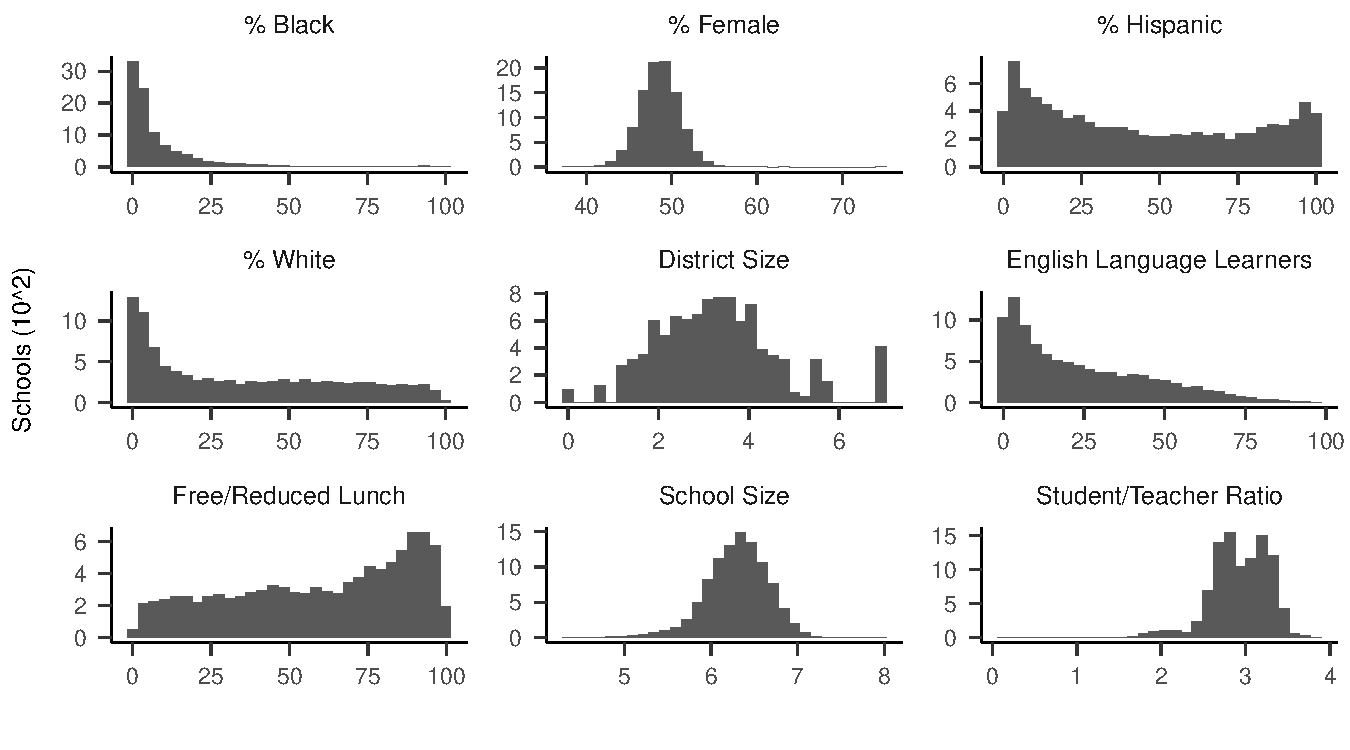
\includegraphics{6---Paper_files/figure-latex/fig-dist1-1.pdf}
\caption{\label{fig:fig-dist1}Distributions of continuous covariates. District Size, N Students, and Student/Teachers were transformed by taking natural logs.}
\end{figure}

\hypertarget{stratification-with-cluster-analysis}{%
\subsection{Stratification with Cluster Analysis}\label{stratification-with-cluster-analysis}}

Cluster analysis serves as a dimension reduction tool to condense the population into smaller set of homogeneous strata. Cluster analysis entails selecting a distance metric, specifying the number of strata, and generating the strata. We describe each of these considerations in turn. All analyses were performed in R (R Core Team, 2017) using the \emph{cluster} package (Mächler, Rousseeuw, Struyf, Hubert, \& Hornik, 2012).

\hypertarget{distance-metric}{%
\subsubsection{Distance metric}\label{distance-metric}}

In a cluster analysis, the distance metric is how dis-similarity between pairs of units on a set of covariates is quantified. As such, the appropriate metric varies depending on the type of data in the matrix.
In educational research contexts, data are likely to contain both continuous and categorical variables, and such was the case here. For mixed data such as this, it is appropriate to use Gower's general similarity measure (Gower, 1971; Tipton, 2013b). This measure relies on different calculations of distance depending on the type of covariates. Let \(x_{pi}\) and \(x_{pj}\) be the observed value of covariate \(p \in \{1, ..., P\}\) for units \(i\) and \(j\) respectively, where \(i \ne j\). Let \(d_{pij}\) be the distance between observed values of covariate \(p\) for sites \(i,j\). For categorical or dummy coded variables, \(d_{pij} = 1\) if \(x_{pi} = x_{pj}\) and \(d_{pij} = 0\) otherwise. For continuous covariates, we use the following formula:
\begin{align}
\label{eq:gowerdist-p}
d_{pij} = 1 - \frac{|X_{pi} - X_{pj}|}{R_p}
\end{align}
where \(|\cdot|\) indicates absolute value and \(R_p\) is the range of observations for covariate \(p\). This equation restricts the range of \(d_{pij}\) to \([0,1]\). We calculated the general similarity between each site pair by taking the weighted average of the distances between all covariates. Let \(d^{g}_{ij}\) be the general similarity between site \(i\) and site \(j\).
\begin{align}
\label{eq:gowerdist}
d^{g}_{ij} = \frac{\sum^P_{p = 1} w_{pij} d_{pij}}{\sum^P_{p = 1} w_{pij}}
\end{align}
where \(w_{pij} = 0\) if \(x_p\) is missing for either site and \(w_{pij} = 1\) otherwise.
We computed a dissimilarity matrix for all \(N \times N\) pairs of units based on the the full set of school-level covariates in Table \ref{tab:tab-RGM-Pars}.

\hypertarget{number-of-strata}{%
\subsubsection{Number of Strata}\label{number-of-strata}}

Selecting an appropriate number of clusters is one of the most difficult problems in cluster analysis (Steinley, 2006). Tipton (2013b) argued that both empirical and practical criteria should be used in selecting \(K\). Hennig and Liao (2013) also argued that the method of selecting \(K\) should depend on the context of the clustering, framing the issue as one of obtaining an appropriate subject-matter-dependent definition rather than a purely statistical question.

Proportional allocation dictates that each stratum should contribute a number of units to the full sample that is proportional to the size of the strata. Having unequal sized strata means that recruiters will need to focus more on larger strata. Generating a larger set of strata would result in greater homogeneity within each stratum, but it may also be more difficult to manage for recruiters. For instance, if refusal and non-response rates are fairly high, having fewer sites spread across more strata may make it difficult to adequately recruit from all strata. Resource constraints (e.g.~time, funding, recruiters) may also be a factor in the number of strata selected.

With these considerations in mind, we examined three criteria for choosing the number of strata: (1) a generalized form of the Calinski-Harabasz index (Cali\a'nski \& Harabasz, 1974) proposed by Hennig and Liao (2013), (2) the proportion of between-cluster variance as recommended by Tipton (2013b), and (3) the practicality of sampling from fewer clusters. Our strategy was to perform the cluster analysis several times for a specified number of clusters, then compare all performance criteria for each set of strata generated (Figure \ref{fig:fig-k-plots}).

We first calculated the Calinski-Harabasz (CH) index using the \emph{cluster.stats} function from the \emph{fpc} (Hennig, 2019) package. Figure \ref{fig:fig-k-plots}a displays the CH index for each \(k\) clusters generated. In this case, generating 2 clusters maximizes the CH-index. Another potential solution is at 4 clusters where there is also a local maxima.



\begin{figure}[tbp]
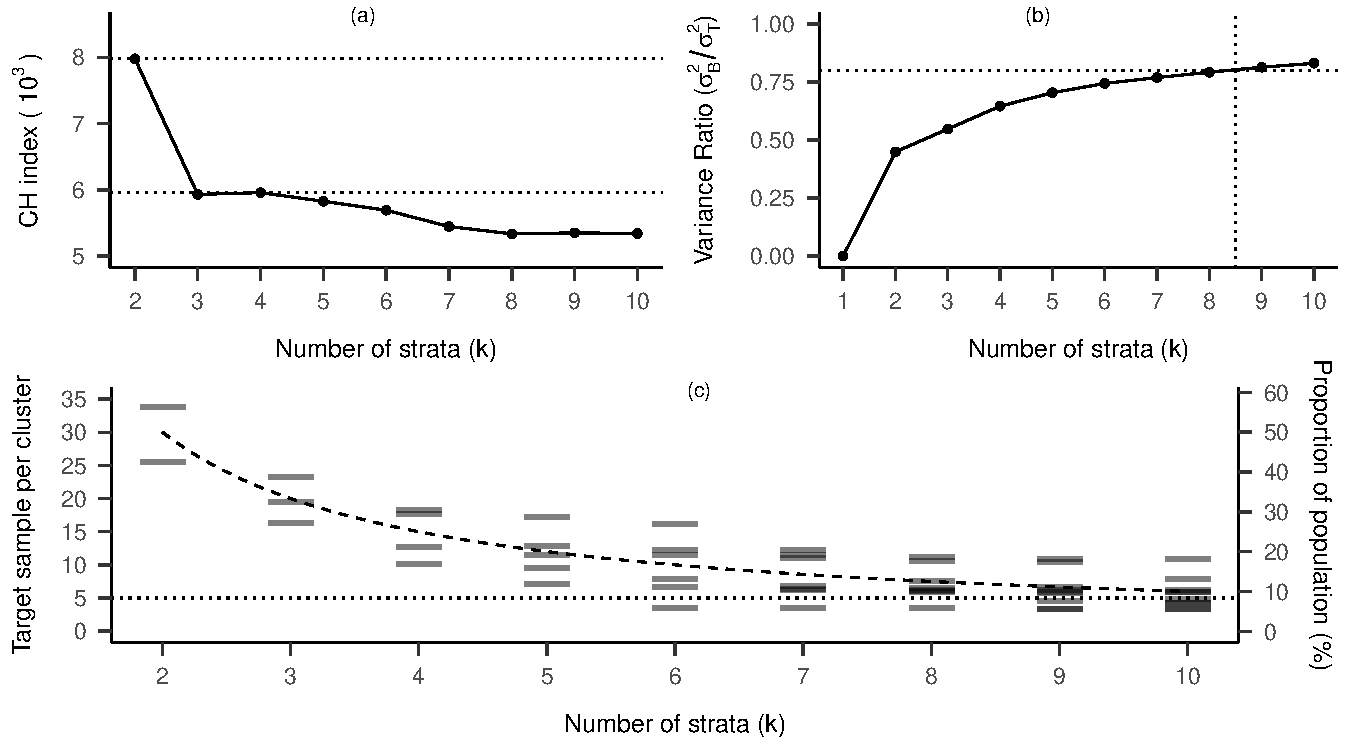
\includegraphics[width=1\linewidth]{6---Paper_files/figure-latex/fig-k-plots-1} \caption{Plots used to determine the number of strata (\(K\)). (a) Calinski-Harabasz index; peaks indicate better fit. (b) Ratio of between cluster sum of squares to total cluster sum of squares; horizontal line indicates cutoff of .8, vertical line indicates minimum number of clusters needed to achieve cutoff. (c) Sampling requirements for each cluster given proportional allocation; horizontal dotted line indicates a minimum sample size requirement of 5 schools. }\label{fig:fig-k-plots}
\end{figure}

We also considered the proportion of variance that lay between clusters. Let \(Q\) be the maximum allowable number of strata. For each set of \(K = 1,..,Q\) strata, we computed the between and within cluster variability for each covariate. We then calculated the proportion of variability that is between strata by taking the sum of the between-cluster variance across all covariates, divided by the sum of the between-cluster and within-cluster variance across all covariates.

Figure \ref{fig:fig-k-plots}b plots \(p_k\) against \(K\). The \(K\) for which the rate of change \(p_k\) slows is considered favorable. Tipton (2013b) also recommended selecting the number of clusters such that at least 80\% of the variability is between clusters; this threshold is indicated in the figure by a dashed line. In light of this criterion, it seems that at least 9 clusters should be generated. However, we also see that after a sharp initial increase, the slope of the graph begins to level out. This indicates that each additional cluster increases the sampling complexity while explaining less variability in covariates. In practice, the difficulty of sampling may not be worth the small increases in homogeneity within clusters obtained when using more than 4 or 5 clusters.

Figure \ref{fig:fig-k-plots}c plots the required sample size from each cluster to fulfill the proportional allocation requirement. The dashed line indicates the ideal allocation if all clusters were of equal size. We see that the variability in cluster sizes decreases as more clusters are generated. A sensible cutoff may be determined by looking at the size of the smallest cluster. When \(K > 5\), the smallest clusters would require less than 5 sites being sampled, which may be very difficult in practice. Considering both the statistical criteria and the pragmatic constraints, we generated 5 clusters for purposes of stratification.

\hypertarget{variation-explained-by-the-strata}{%
\subsection{Variation explained by the strata}\label{variation-explained-by-the-strata}}

The strata resulting from the cluster analysis range in size from XX to XX schools. The strata explain XX\% of the variation across all covariates (Figure \ref{fig:fig-k-plots}b), with a CH-index of XX (Figure \ref{fig:fig-k-plots}a).\todo[color=blue!20]{Complete this sub-section with details about variation explained in individual covariates. This should set up Figure 5 in the results.}

\hypertarget{simulating-sample-recruitment}{%
\section{Simulating sample recruitment}\label{simulating-sample-recruitment}}

Using the formal models for unit participation and sample recruitment that we have described, it becomes possible to simulate the process of recruiting schools for an MRT.
Monte Carlo simulations, such as the one we now describe, are a flexible method for assessing the performance of different sample recruitment methods under controlled conditions.
Here, we use simulation to assess the generalizability of samples recruited through SBS relative to probability sampling or convenience sampling methods. We also examine the feasibility and equity with which the sampling methods can be employed.

The validity and utility of a simulation study rests on whether the models and assumptions employed are reasonable approximations to the processes involved in collecting real data. In particular, our simulation findings rest on the assumptions of the participation propensity model and recruitment models. By relying on previous work and real data to inform our modeling assumption, we hope to reasonably represent trends in the performance of different recruitment methods. That said, given the speculative nature of some aspects of the simulation our conclusions are tentative.\todo[color=blue!20]{I would not claim that we are representing reality here. Need a big "however" to conclude this paragraph...} \todo[color=orange]{Added}

\hypertarget{data-generation}{%
\subsection{Data Generation}\label{data-generation}}

\hypertarget{population-and-strata}{%
\subsubsection{Population and Strata}\label{population-and-strata}}

We study the performance of different recruitment methods for a study aimed at generalizing to the population of schools in six states, as described in the previous section. For recruitment methods involving stratification, we use the five strata generated through the cluster analysis of the school and student characteristics listed in Table \ref{tab:tab-RGM-Pars}.
Because these strata are a function of the characteristics of the full population, they are fixed and constant across replications of the simulation and across the different conditions that we examine.

\hypertarget{participation-propensity-score}{%
\subsubsection{Participation Propensity Score}\label{participation-propensity-score}}

We modeled the participation propensity score (Equation \eqref{eq:RGM}) using parameter estimates from extant school data. The set of covariates consisted of the same variables used in the cluster analysis. The corresponding coefficients were based on work by Fellers (2017) who compared 571 elementary schools that participated in IES funded studies to the full population of U.S. elementary schools. The authors reported absolute SMD between the schools that participated and the population. We standardized the covariates and used reported SMDs as coefficients in Equation \eqref{eq:RGM} to generated \(\pi_j\) values. The coefficient values are reported in Table \ref{tab:tab-RGM-Pars}.

The results of Fellers (2017) do not provide any information about the overall average participation propensity across the full population--that is, the fraction of the full population of schools that would agree to participate in a study, if approached. This is a key parameter of the simulation that has a strong influence on the performance of all recruitment methods. We therefore varied the overall participation propensity over a wide range, by manipulating the intercept term in Equation \eqref{eq:RGM}. We considered nine different levels of participation rates, ranging from 10\% to 90\%.

\hypertarget{simulation-procedures}{%
\subsection{Simulation procedures}\label{simulation-procedures}}

We designed the simulation to examine the performance of 5 recruitment methods across 9 levels of population participation. The population of schools and their assigned strata were constant across all conditions and replications. The participation propensity score was constant across all sampling methods and replications within each level of population participation. Each replication involved first simulating potential participation indicators (\(E_j\)'s) according to Equation \eqref{eq:Ej}, which we then treated as constant across each sampling method. That is, if a given school was selected in each of three sampling methods, the school would provide the same response for all three methods, either agreeing or refusing to participate. Next, we generated five sets of rankings (one for each recruitment method) for all schools.
We checked each school in order of rank for recruitment until a sample of 60 schools was selected by each method. For each sample within an iteration, we tracked which schools agreed to participate, which schools refused to participate, and how many schools refused to participate.
The order in which schools were approached varied by recruitment method and across replications. The one exception was the stratified balanced sampling method, where the order in which schools are approached is constant because it is a function of stratum assignment and school characteristics.

\hypertarget{performance-measures}{%
\subsection{Performance measures}\label{performance-measures}}

\hypertarget{generalizability}{%
\subsubsection{Generalizability}\label{generalizability}}

There are several methods to quantify how generalizable a sample is to a target population. One common method is to compare the sample to the population on a range of covariates by examining SMDs as shown in Equation \eqref{eq:SMD}. This method is limited as it only provides us with a measure of how close the sample means are to the population means.
To have true generalizability, however, we must also account variance representation. \todo[color=blue!20]{Couldn't we just compare variance ratios then? More positive justification for the B index?} \todo[color=orange]{added}

A more comprehensive method is to calculate a generalizability index (\(B\); Tipton, 2014) which provides a single score summary of overlap between two groups. This index offeres several advantages, First, it takes into account both the variance and distribution of the variables in each group by measuring the overlap of multiple density plots. Second, it quantives what is typically a visual comparison and provides an intuitive interpretation. Third, it simulatniously compares two groups across a range of covariates and can easily be scaled to include various interactions and transformations. This is done using propensity score analysis to estimating a summary statistic that represents differences between groups.

The first step is to perform a propensity score analysis. Let \(\hat\psi_j\) represent the sample propensity score, or the probability that school \(j\) was included in a given sample. We estimate \(\hat\psi_j\) using a basic logistic regression:

\begin{align}
\label{eq:PSA}
\hat\psi_j = \log\left(\frac{\pi_j}{1 - \pi_j}\right) = \beta_0 + \mathbf{x}_j \boldsymbol\beta + e_j
\end{align}

This is essentially the reverse of the participation generation model (equation \eqref{eq:RGM}) where instead of generating a propensity to participate for each school, we are now estimating the propensity of each school actually participating when implementing a given sampling method. Here, \(\hat\psi_j\) serves as a scalar summary of differences across all covaraites in \(\mathbf{x}_j\). \todo[color=blue!20]{Details about estimated propensity score.}\todo[color=orange]{added, please look over}

We then calculate the generalizability index to compare the distribution of \(\hat\psi_j\) in the sample to that of the population.
The generalizability index is bounded between 0 and 1, with 0 indicating no overlap between the sample and the population, and 1 indicating the sample is representative of the population.
Given the estimated propensity scores \(\hat\psi_1,...,\hat\psi_N\), we calculated the \(B\) index as
\begin{align}
B = \int_{\hat\psi_{min}-3h_{max}}^{\hat\psi_{max}+3h_{max}}\sqrt{\hat{f}_s(z)\hat{f}_p(z)}dz
\end{align}
where \(\hat\psi_{min}\) and \(\hat\psi_{max}\) are the minimum and maximum values of \(\hat\psi\) respectively, \(\hat{f}_s(z)\) is a Gaussian kernel density estimate of the distribution of propensity scores in the sample, calculated using bandwidth \(h_s\), and \(\hat{f}_p(z)\) is a Gaussian kernel density estimate of the distribution of propensity scores in the non-sampled population, calculated using bandwidth \(h_p\). We calculated the bandwidth \(h\) for the population or sample as follows:
\begin{align}
h = \sigma_{\pi}\left(\frac{4}{3n}\right)^{1/5}
\end{align}
where \(\sigma_{\pi}\) is the standard deviation of the propensity scores.

\hypertarget{feasibility}{%
\subsubsection{Feasibility}\label{feasibility}}

Recruiters expend a lot of resources contacting districts and schools, scheduling meetings and traveling between prospective schools. A project with limited resources may not be able to afford to go through a large list of potentially uninterested schools. To capture the feasibility of different recruitment methods, we tracked the total number of schools approached to achieve a full sample.\todo[color=blue!20]{Add Equation numbers} We then calculated the average number of refusals needed to achieve a full sample for each recruitment method. This measure allows us to compare the feasibility or difficulty of recruiting a full sample by each method.

\hypertarget{sampling-inequity}{%
\subsubsection{Sampling Inequity}\label{sampling-inequity}}

\todo[color=blue!20]{Start with the rationale/motivation for looking at inequity.} To assess sampling inequity, we tracked the frequency with which schools were recruited by each method. We then summarized these data by calculating a Gini coefficient for each recruitment method and each population participation rate. This index ranges from 0 to 1, with 0 indicating perfect equity, and 1 indicating total inequity. In economic contexts, the Gini coefficient is used to describe the degree of income inequality by showing the disproportionate distribution of wealth across levels of incomes. Similarly it could be used in the context of sampling by identifying how often under-represented schools are recruited to participate in studies. We calculated Gini coefficients using the \emph{Gini} function from the \emph{ineq} package (Zeileis 2014).

\hypertarget{results}{%
\section{Results}\label{results}}

\hypertarget{generalizability-1}{%
\subsection{Generalizability}\label{generalizability-1}}

\hypertarget{b-index}{%
\subsubsection{B-Index}\label{b-index}}

Figure \ref{fig:fig-avg-B} displays the average \(B\)-index for each method across participation rates.\todo[color=blue!20]{Couldn't figure out how to get the Figure to the top of the page.} Acceptable values of \(B\) for generalizability vary depending on the size of the sample, the size of the population, and the number of covariates (Tipton, 2014). Given our design, a value of \(B = .95\) would indicate very good overlap with no need to adjust estimates. Generally \(B >= .80\) still supports generalizability with adjustment and likely no need to redefine the population. At population participation rates below 40\%, SBS consistently out-performed the other recruitment methods. Further, across population response rates, SBS never resulted in a \(B\) value below .85. This indicates that SBS is successful at sampling schools that are unlikely to participate and therefore tend to be underrepresented by the other sampling methods---particularly when overall participation propensities are low. Stratified random sampling consistently outperformed simple random sampling across all participation rates, though only slightly.\todo[color=blue!20]{For all of the figures in this section, I think it would better to combine the two dimensions of the legends so that color AND line have values of SBS, SRS, URS, SCS, UCS. Double encoding will help with black-and-white legibility. Might also need to add geom\_point with shape corresponding to recruitment method, and/or get rid of the legend and just directly label the lines (try geom\_label\_rapel from ggrepel pkg).}



\begin{figure}
\centering
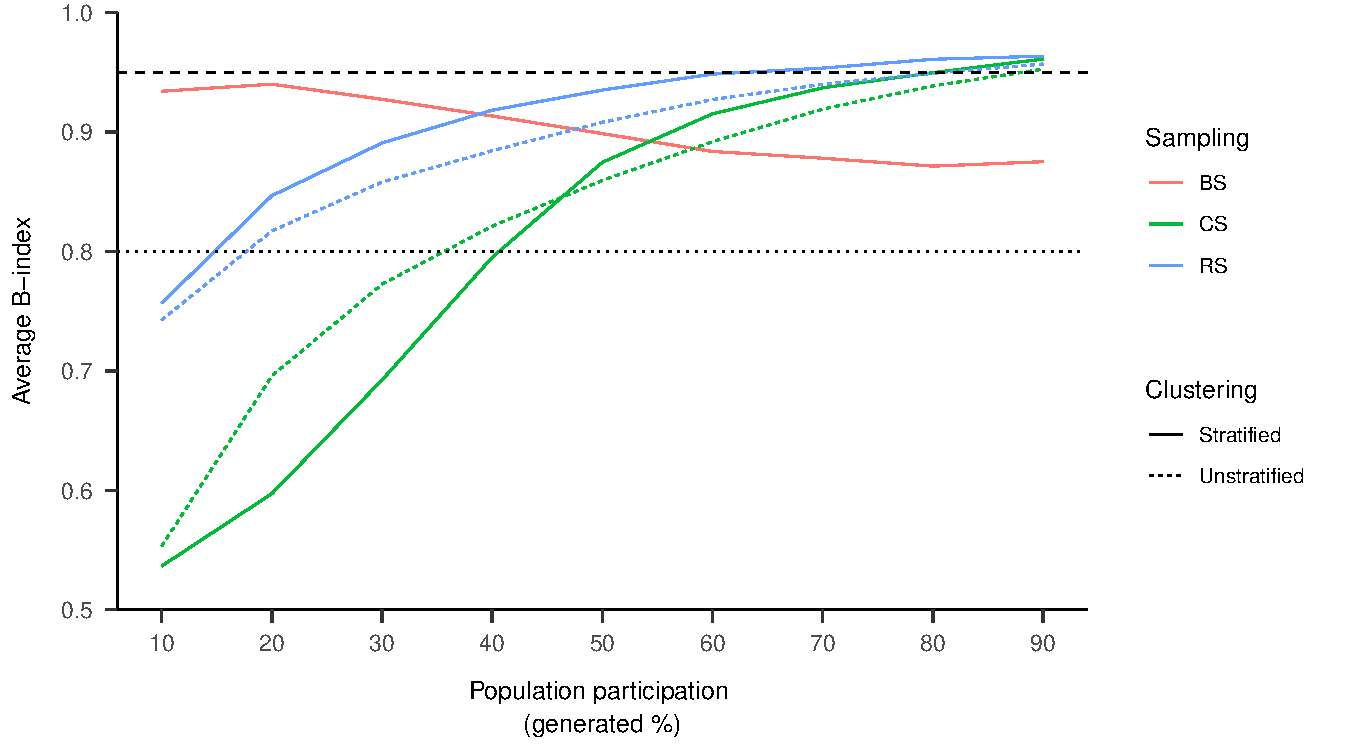
\includegraphics{6---Paper_files/figure-latex/fig-avg-B-1.pdf}
\caption{\label{fig:fig-avg-B}Average \(B\)-index for varying participation rates, by sampling method. Horizontal dotted and dashed lines represented indices of .80 and .95, respectively, indicating acceptable or high levels of generalizability.}
\end{figure}

We also found several trends that were unexpected. At 50\% and beyond, SBS performance slowly degraded, while other methods maintained a steady increase. We expected a constant positive relationship between the population participation rate and the performance of all methods. Furthermore, at low response rates, unstratified convenience sampling achieved better balance than stratified convenience sampling. This seems counter-intuitive, as survey literature suggests that stratified samples are more representative.\todo[color=blue!20]{Cite} Because the B-index is an overall measure of generalizabilty across many covariates, it does not provide much indication of why these performance differences occur. To untangle why the methods performed as they did, we need to examine the balance obtained by each recruitment method on individual covariates.

\hypertarget{standardized-mean-differences}{%
\subsubsection{Standardized Mean Differences}\label{standardized-mean-differences}}

We began this analysis by plotting mean SMDs for each recruitment method on each individual covariate versus the population participation rate. We considered a method to perform well if it resulted in an average imbalance of no more than 0.25 standard deviations. The relative performance of sampling methods varied depending on the covariate. Several patterns did emerge, based on which we identified three groups of covariates. Figure \ref{fig:fig-SMD-groups} displays an example of each pattern; results for specific covariates can be found in Online Appendix Figure XX.\todo[color=blue!20]{Fill in.} The first group of covariates included nine variables where stratified methods outperformed unstratified methods at every population participation rate. The second group included two covariates where all sampling methods resulted in good balance. The third group included three covariates where where at least one unstratified method performed better than the corresponding stratified method. Across all groups, stratified balanced sampling almost always resulted in acceptable balance and generally yielded better balance than all other sampling methods.



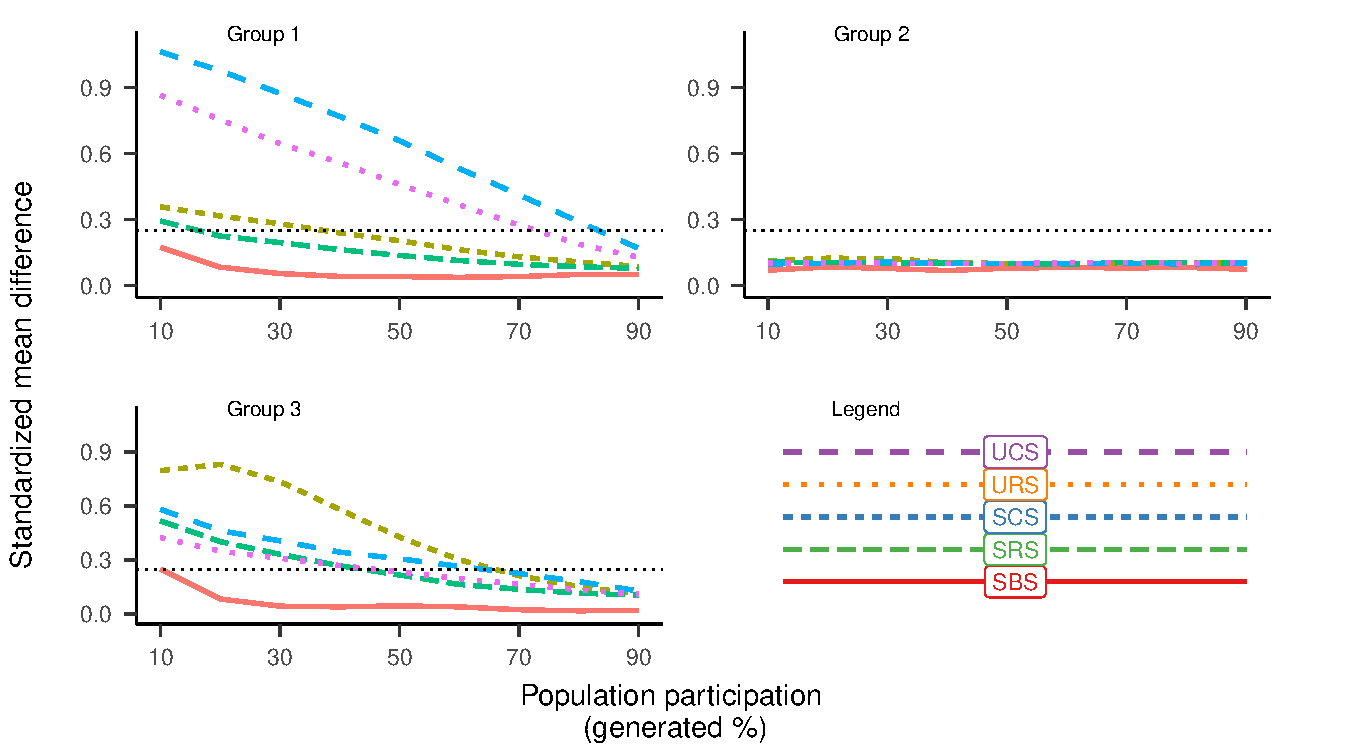
\includegraphics{6---Paper_files/figure-latex/unnamed-chunk-1-1.pdf}

One potential explanation the patterns found in groups 2 and 3 is that the strata were poorly specified for these covariates. To examine this we calculated the the proportion of variance explained by the strata for each covariate and compared it to the log-odds coefficients associated with that covariate in the participation propensity model (Figure \ref{fig:fig-Var-Coef}). Several patterns emerged here as well. Group 1 consisted of covariates where a substantial fraction of the variance was between clusters. Groups 2 and 3 both consisted of covariates that were poorly clustered, with no more than 15\% of variance between clusters. The major difference between groups 2 and 3 appears to be the relationship between the covariates and the likelihood of participation.\todo[color=blue!20]{2-3 sentences of explanation of how these findings relate to overall patterns from previous figure.}



\begin{figure}
\centering
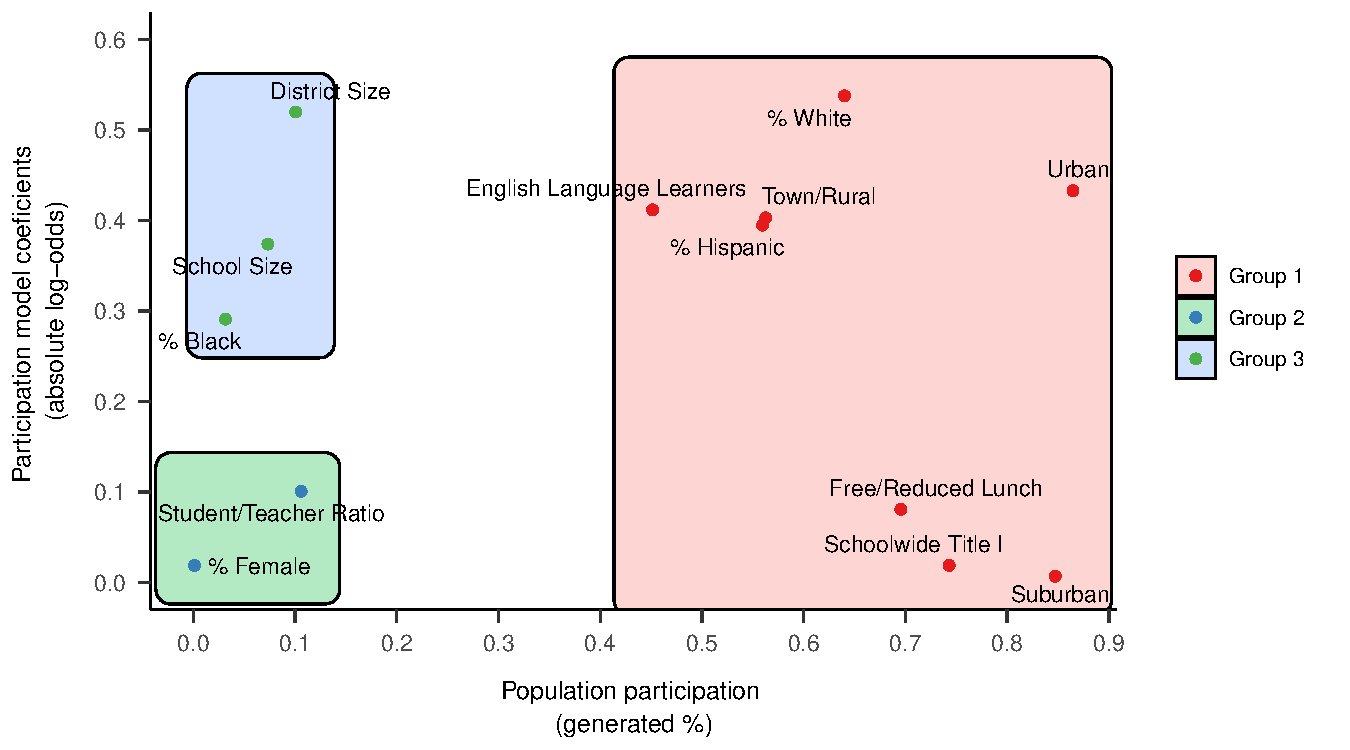
\includegraphics{6---Paper_files/figure-latex/fig-Var-Coef-1.pdf}
\caption{\label{fig:fig-Var-Coef}Variance explained by clustering vs absolute log odds. Shaded areas illustrate patterns in generalizability measured by SMDs.}
\end{figure}

\hypertarget{feasibility-1}{%
\subsection{Feasibility}\label{feasibility-1}}

\hypertarget{recruitment-attempts}{%
\subsubsection{Recruitment Attempts}\label{recruitment-attempts}}

Figure \ref{fig:fig-responses}a depicts the total number of schools contacted to recruit a full sample of 60 schools versus the population participation rate, for each recruitment method. Figure \ref{fig:fig-responses}b depicts the response rate, or percentage of schools that agreed to participate among those where recruitment was attempted, versus the population participation rate, for each recruitment method.\todo[color=blue!20]{Vertical axis should be "Participation response rate."} For each of these metrics, there were substantial differences between methods at lower population participation rates.\todo[color=blue!20]{Add a few sentences summarizing differences between methods. How does BS compare to CS, CS to RS, stratified versus not, etc.?} At higher participation rates, the differences were less pronounced, becoming negligible at population participation rates of 60\% or more.

It is important to note that the magnitudes of these results are quite extreme.\todo[color=blue!20]{What aspect of the results?} This is likely due to some mis-specification on the part of the simulation either in the response generating model parameters or the population participation rates. Rather than looking at the raw values, a more meaningful interpretation would be to compare the relative performance of the recruitment methods. Overall, UCS required the smallest recruitment effort to obtain a full sample, followed by URS and SCS, SRS, and finally SBS.\todo[color=blue!20]{Let's discuss this paragraph. Not sure about suggesting mis-specification here.}



\begin{figure}
\centering
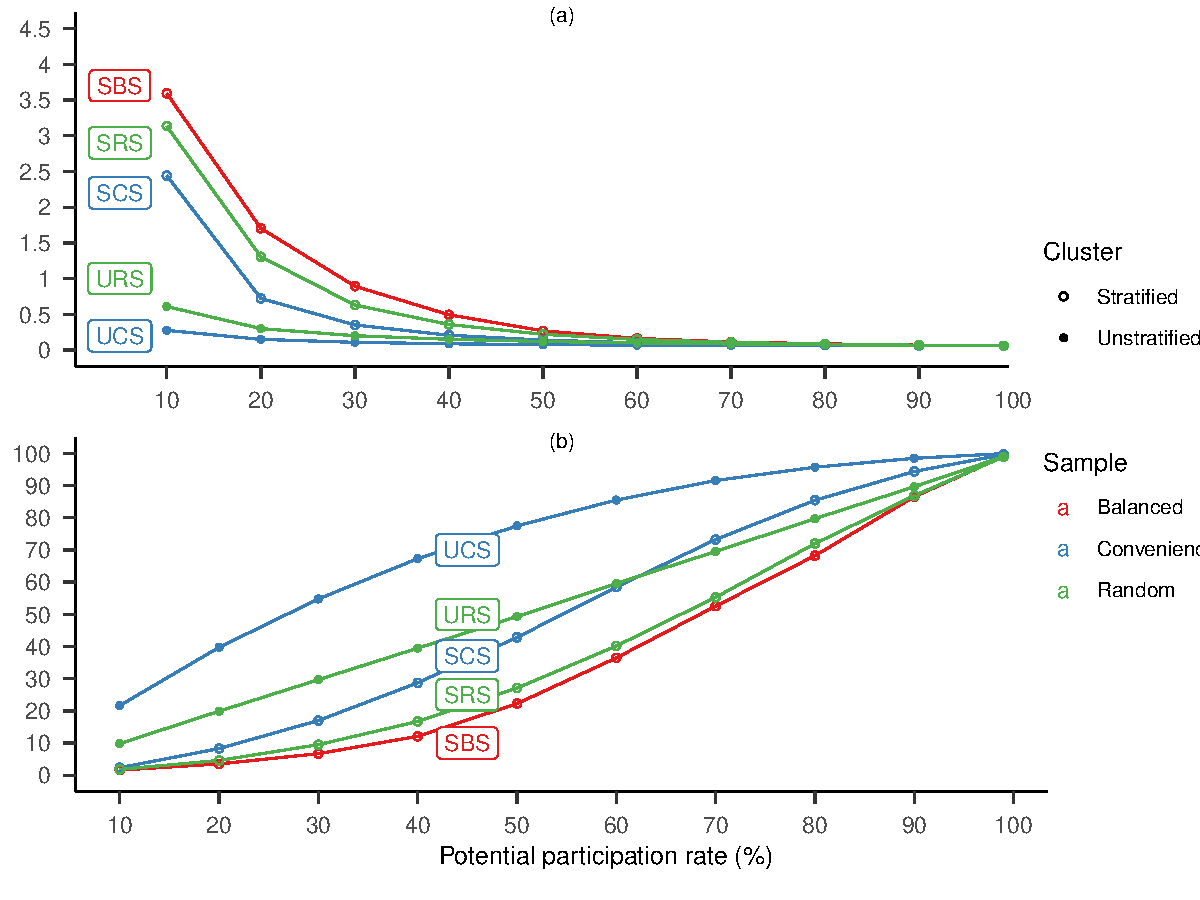
\includegraphics{6---Paper_files/figure-latex/fig-responses-1.pdf}
\caption{\label{fig:fig-responses}Sample recruitment statistics and response rates. Plot (a) shows the total number of units contacted to achieve a full sample of 60 schools. Plot (b) shows the percent of schools that agreed to participate when recruited.}
\end{figure}

\hypertarget{sampling-inequity-1}{%
\subsubsection{Sampling Inequity}\label{sampling-inequity-1}}

We calculated the Gini coefficient for each sampling method to examine the equity implications of different recruitment methods. Figure \ref{fig:fig-gini} displays these for each sampling method across population participation rates. A coefficient of 1 indicates absolute sampling inequity. In the context of the simulation, a high Gini coefficient indicates that across replications, only a small subset of the population was ever actually recruited.\todo[color=blue!20]{Recruited or participated?}

Several trends emerged in this analysis. As population participation rates increased, inequity increased when using SBS, but decreased when using any other method. These four other methods also performed consistently relative to one another, with SRS resulting in the least amount of sampling inequality, followed by URS, SCS and UCS. As population rates increased, differences between stratified and unstratified versions of sampling methods seemed to decrease. This finding suggests that stratifying the population results in a larger potential sampling pool when the overall population response rate is low.\todo[color=blue!20]{Revise the full paragraph, starting by explaining overall differences across methods. Which methods led to less equitable participation? What's the headline? Then talk about patterns across different population participation rates.}



\begin{figure}
\centering
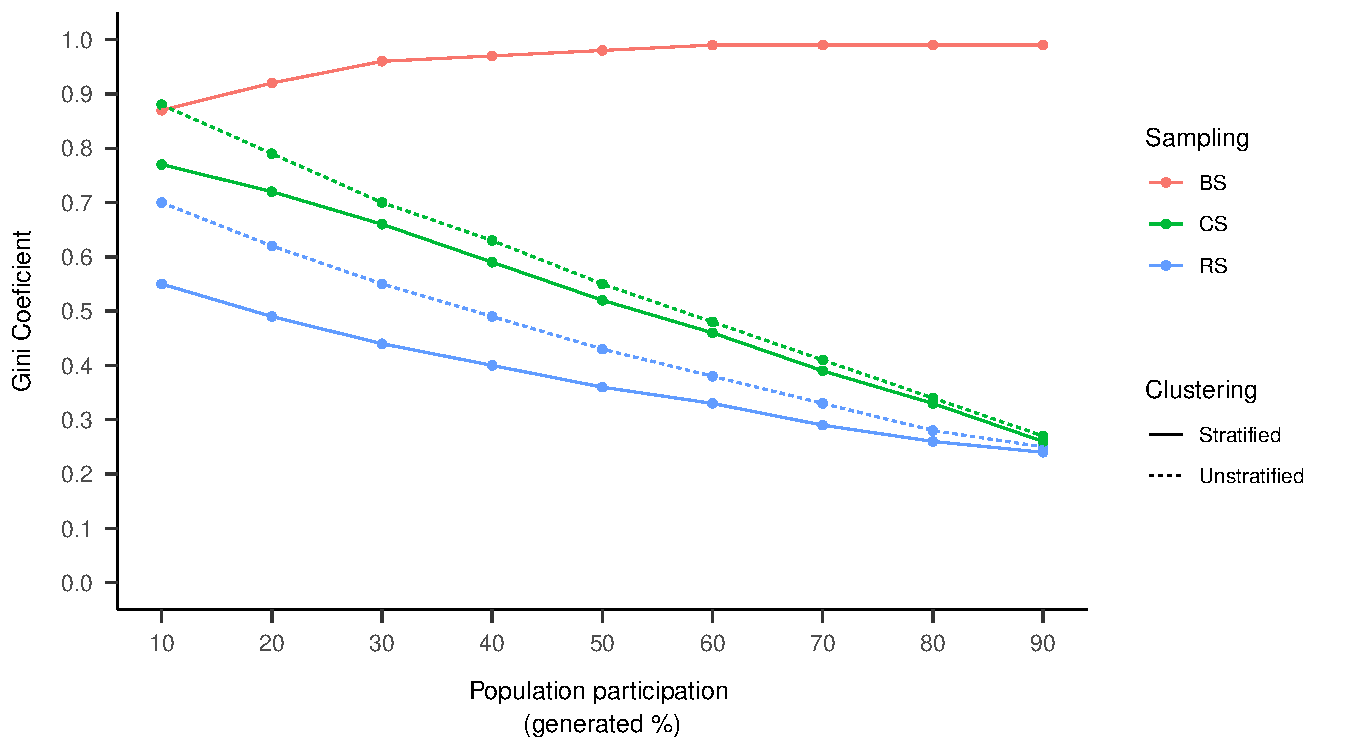
\includegraphics{6---Paper_files/figure-latex/fig-gini-1.pdf}
\caption{\label{fig:fig-gini}Gini coefficient across participation response rates for each sampling method. A coefficient of 1 indicates major inequality in sampling probability.}
\end{figure}

\hypertarget{summary-of-trends}{%
\subsection{Summary of Trends}\label{summary-of-trends}}

Under the assumptions of our simulation models, recruiting samples using SBS yielded highly generalizable samples. In particular, SBS resulted in a considerable improvement compared to UCS---the method that we suspect most closely approximates current practice. However, given the large number of schools contacted to obtain a full sample, it may be infeasible to fully implement SBS in the ideal form. Another consistent pattern was that convenience and probability sampling methods were often improved by first stratifying the population. In certain cases,\todo[color=blue!20]{Be specific about which cases} convenience sampling within strata (SCS) performed comparably to simple random sampling (URS) both in terms of generalizability and feasibility.

A further pattern in these simulation results relates the specification of the clustering method to the response model. For instance, in Figure \ref{fig:fig-SMD-group4} we see that all methods of sampling result in balance on percentage of Black students, except for stratified convenience sampling. This is likely a result of the covariate having a strong relationship with participation, but not being weighed enough in the cluster analysis used in determining the strata. Figure \ref{fig:fig-Var-Coef} displays the calculated intraclass correlation coefficient (ICC) for each covariate along the strata, and the coefficient for each covariate in the response generating model. For covariates where one value (ICC or coefficient) is high, while the other is low, stratified sampling techniques resulted in poorer balance.\todo[color=blue!20]{This paragraph is very in-the-weeds. What is the high level summary and what is the implication?}

\hypertarget{discussion}{%
\section{Discussion}\label{discussion}}

The main goal of this study was to develop a framework for exploring the performance of different recruitment methods within the context of multi-site trials in education research. We have described several models for algorithmically representing how researchers might select samples of schools. Drawing on prior empirical work, we also attempted to model how schools may decide whether or not to participate in a study if approached by recruiters. The methods we proposed for modeling these behaviors can, in principle, be extended to more complex and realistic specifications and adapted to other population frames.

A second goal was to use this framework to investigate the relative perfomance of different several sampling methods in terms of generalizability and feasibility. Based on these simulation, we draw several tentative conclusions. Stratified balanced sampling as proposed by Tipton (2013b) has the potential to greatly increase the generalizability of samples selected for MRTs. However, this method is not without limitations. Within our simulation, strict application of SBS came at a great cost in terms of the number of schools that needed to be contacted. Thus, implementing this method in practice may require allocating many more study resources to sample recruitment.

We also found that the properties of the strata generated by cluster analysis have implications for the generalizability of samples recruited through stratified methods. If a covariate was predictive of participation propensity, then it was important for the stratification to explain a substantial fraction of its total variation. If a covariate was predictive of participation, but not prioritized when generating the strata, it had poor representation in samples collected through stratified methods. Ignoring the the quality of the cluster analysis solution has the potential to undermine the performance of SBS. Finally, while the balanced sampling approach does result in strong generalizability, it might also limit the pool of potential participants. Particularly for larger population response rates, the same subset of schools were likely to be recruited across replications of the simulation.

One potential compromise between current practice (such as UCS) and SBS is to combine stratification with some form of convenience sampling. As demonstrated in the simulations, stratified convenience sampling often resulted in better balance on individual covariates than simple random sampling. This may also elicit greater buy in from recruiters by placing less restrictions on which units they must sample.\todo[color=blue!20]{What about relative feasibility?}
Beyond generalizability, stratifying in this manner requires that researchers make sampling decisions in the study design phase, and to track changes in the sampling plan as recruitment progresses. Documenting and reporting this process would in turn support further research into developing more efficient and effective sampling methods.

\hypertarget{limitations}{%
\subsection{Limitations}\label{limitations}}

The models that we have studied make several key assumptions which represent limitations on the findings from the simulation study. First, in modeling convenience sampling, we assumed that recruiters always prioritize schools that are most likely to participate. In reality, other factors may play a role as well, such as proximity of sample sites to the researcher and to each other, existing relationships between the recruiters and the sample sites, and other researcher assumptions about the sample site's characteristics.\todo[color=blue!20]{Not sure what you mean by the last one.} This limits how well our results capture the absolute performance and feasibility of convenience sampling methods.

Another implication of this assumption is that recruiters have approximate knowledge of how likely a sampled site is to participate. Though researchers may speculate about sites that are more willing to participate (such as schools in larger urban districts) and prioritize recruiting such sites, their estimation of \enquote{willingness} may be further from the truth than what we have assumed. If so, it is possible that the feasibility of the convenience methods is over-stated and that their degree of generalizability is under-stated.

It would be worth refining and exploring additional methods for modeling convenience sampling. The algorithms used in these methods could be tuned to include additional factors that might influence school recruitment priorities. For instance, location data is readily available and could be incorporated into the model for how researchers prioritize schools in convenience sampling. Further work here could lead to more realistic and practical assessments of feasibility and generalizabilty, potentially providing researchers with a tool for evaluation of recruitment methods given the unique circumstances that they face during the study design phase.

A second limitation arises from the simplified and speculative nature of our participation model. In practice, the decision of whether a school participates in such a study often involves multiple stages. District offices often serve as gatekeepers, requiring submission and approval of research requests prior to starting recruitment of individual schools. If the request is denied, no schools within the district may be recruited. If approved, researchers may work with a district-wide school coordinator, or may have to contact schools individually. In either cases, the ultimate decision may then rest with administrators, school research coordinators, or the teachers themselves.\todo[color=blue!20]{Implications for our findings?}

A further limitation of the simulations is that the parameters in the response generating model are based on values from a study that examined the difference between schools participating in large-scale RCTs and the overall population of schools. However, these RCTs themselves typically rely on some form of convenience sampling. Consequently, our parameters reflect participation rates of schools that are likely to participate in RCTs, rather than the full population of schools.

This limitation points towards the need for more extensive research regarding factors that influence school participation in RCTs. In particular, research is needed that can disentangle recruitment bias from selection bias. Such information could be generated through careful record-keeping during the recruitment stages of MRTs, particularly if the recruitment methods are operationally defined and if the study aims for large-scale population representation.
Such efforts could provide deeper insight into school behavior and representation in research. If we can identify schools that are consistently and systematically under-represented in funded research, we can develop strategies to target such schools and increase the inclusivity of studies that strive for truly representative population-level inferences.

\hypertarget{future-directions}{%
\subsection{Future Directions}\label{future-directions}}

In this study, we have sought to lay the groundwork for several avenues of further research. First, additional work is needed on how best to implement cluster analysis in the context of stratified sampling methods. We have shown that the extent to which balance is achieved on a given covariate is related to how strongly the strata explain variation in the covariate and how strongly the covariate is related to school participation. If some covariates are known to have greater influence on school participation, it may be useful to weight them more heavily in generating the strata. Further work is also needed to understand the relationship between the number of strata, generalizability, and feasibility. It is expected that more clusters would increase generalizability, but also make recruitment more difficult. A better understanding of these relationships would help drive decision-making during the design phase, potentially making SBS more accessible and quicker to implement.

Further work also needs to examine the impact of these sampling methods on the bias and accuracy of population average treatment effect estimates. In this study, our goal was only to select a generalizable sample, where generalizability was operationalized as balance between the sample and population on a set of covariates. To the extent that the same covariates that dictate selection are also predictive of variance in treatment effects, we may extrapolate that a sample that is balanced on these covariates can be used to estimate an unbiased PATE. Still, we think it would be worth investigating the full process--from study design to parameter estiamtion--to understand how sampling methods might influence the bias in impact estimates for a target population.

If treatment effects are constant across units in a population, non-representative samples of the population should still lead to unbiased estimates of average treatment effects. However, if only a narrow slice of the population is studied, there may not be sufficient variability in potential moderators to detect heterogeneity. Adding variation by selecting a more diverse sample may be useful if the extent of heterogeneity is unknown. This further complicates the specification of the cluster analysis. How should covariates be weighed relative to each other depending on whether they predict participation, differences in treatment effects, or some combination of both? To address this our work must be extended to study the relationship between sampling methods and bias in treatment effect estimation.\todo[color=blue!20]{I don't quite follow how this fits in. Let's discuss this point.}

Large scale MRTs are expensive to implement, and resource allocation for such studies presents many difficult trade-offs. Researchers who wish to invest in robust recruitment strategies to amplify the impact and relevance of of their work should be better equipped to anticipate the costs and benefits of various sampling strategies. Through further refinement of the models and simulations demonstrated here, we hope to help researchers make more informed decisions about sample recruitment and representation.

\newpage

\hypertarget{references}{%
\section{References}\label{references}}

\begingroup
\setlength{\parindent}{-0.5in}
\setlength{\leftskip}{0.5in}

\hypertarget{refs}{}
\leavevmode\hypertarget{ref-calinskiDendriteMethodCluster1974}{}%
Cali\a'nski, T., \& Harabasz, J. (1974). A dendrite method for cluster analysis. \emph{Communications in Statistics}, \emph{3}(1), 1--27. \url{https://doi.org/10.1080/03610927408827101}

\leavevmode\hypertarget{ref-fellersDevelopingApproachDetermine2017}{}%
Fellers, L. (2017). \emph{Developing an approach to determine generalizability: A review of efficacy and effectiveness trials funded by the Institute of Education Sciences} (Ph.D.). Columbia University, United States -- New York. Retrieved from \url{https://search.proquest.com/docview/1865595768/abstract/40FD82F4A0C24535PQ/1}

\leavevmode\hypertarget{ref-gerberFieldExperimentsDesign2012}{}%
Gerber, A. S., \& Green, D. P. (2012). \emph{Field experiments: Design, analysis, and interpretation} (1st ed). New York: W. W. Norton.

\leavevmode\hypertarget{ref-gowerGeneralCoefficientSimilarity1971}{}%
Gower, J. C. (1971). A General Coefficient of Similarity and Some of Its Properties. \emph{Biometrics}, \emph{27}(4), 857--871. \url{https://doi.org/10.2307/2528823}

\leavevmode\hypertarget{ref-grovesSurveyMethodology2004}{}%
Groves, R. M. (Ed.). (2004). \emph{Survey methodology}. Hoboken, N.J: Wiley-Interscience.

\leavevmode\hypertarget{ref-R-fpc}{}%
Hennig, C. (2019). \emph{Fpc: Flexible procedures for clustering}. Retrieved from \url{https://CRAN.R-project.org/package=fpc}

\leavevmode\hypertarget{ref-hennigHowFindAppropriate2013}{}%
Hennig, C., \& Liao, T. F. (2013). How to find an appropriate clustering for mixed-type variables with application to socio-economic stratification: How to Find an Appropriate Clustering. \emph{Journal of the Royal Statistical Society: Series C (Applied Statistics)}, \emph{62}(3), 309--369. \url{https://doi.org/10.1111/j.1467-9876.2012.01066.x}

\leavevmode\hypertarget{ref-imaiMisunderstandingsExperimentalistsObservationalists2008}{}%
Imai, K., King, G., \& Stuart, E. A. (2008). Misunderstandings between experimentalists and observationalists about causal inference. \emph{Journal of the Royal Statistical Society: Series A (Statistics in Society)}, \emph{171}(2), 481--502. \url{https://doi.org/10.1111/j.1467-985X.2007.00527.x}

\leavevmode\hypertarget{ref-kernAssessingMethodsGeneralizing2016}{}%
Kern, H. L., Stuart, E. A., Hill, J., \& Green, D. P. (2016). Assessing Methods for Generalizing Experimental Impact Estimates to Target Populations. \emph{Journal of Research on Educational Effectiveness}, \emph{9}(1), 103--127. \url{https://doi.org/10.1080/19345747.2015.1060282}

\leavevmode\hypertarget{ref-lohrSamplingDesignAnalysis2019}{}%
Lohr, S. L. (2019). \emph{Sampling: Design and Analysis} (2nd Edition). Chapman and Hall/CRC.

\leavevmode\hypertarget{ref-machlerClusterClusterAnalysis2012}{}%
Mächler, M., Rousseeuw, P., Struyf, A., Hubert, M., \& Hornik, K. (2012). \emph{Cluster: Cluster Analysis Basics and Extensions} (Vol. 1).

\leavevmode\hypertarget{ref-olsenExternalValidityPolicy2013}{}%
Olsen, R. B., Orr, L. L., Bell, S. H., \& Stuart, E. A. (2013). External Validity in Policy Evaluations That Choose Sites Purposively. \emph{Journal of Policy Analysis and Management}, \emph{32}(1), 107--121. \url{https://doi.org/10.1002/pam.21660}

\leavevmode\hypertarget{ref-omuircheartaighGeneralizingUnrepresentativeExperiments2014}{}%
O'Muircheartaigh, C., \& Hedges, L. V. (2014). Generalizing from unrepresentative experiments: A stratified propensity score approach. \emph{Journal of the Royal Statistical Society: Series C (Applied Statistics)}, \emph{63}(2), 195--210. \url{https://doi.org/10.1111/rssc.12037}

\leavevmode\hypertarget{ref-raudenbush2015learning}{}%
Raudenbush, S. W., \& Bloom, H. S. (2015). Learning about and from a distribution of program impacts using multisite trials. \emph{American Journal of Evaluation}, \emph{36}(4), 475--499.

\leavevmode\hypertarget{ref-raudenbushStatisticalPowerOptimal2000}{}%
Raudenbush, S. W., \& Liu, X. (2000). Statistical power and optimal design for multisite randomized trials. \emph{Psychological Methods}, \emph{5}(2), 199--213. \url{https://doi.org/10.1037//1082-989X.5.2.199}

\leavevmode\hypertarget{ref-rcite}{}%
R Core Team. (2017). \emph{R: A language and environment for statistical computing}. Vienna, Austria: R Foundation for Statistical Computing. Retrieved from \url{https://www.R-project.org/}

\leavevmode\hypertarget{ref-shadishExperimentalQuasiexperimentalDesigns2002}{}%
Shadish, W. R., Cook, T. D., \& Campbell, D. T. (2002). \emph{Experimental and quasi-experimental designs for generalized causal inference}. Boston, MA, US: Houghton, Mifflin and Company.

\leavevmode\hypertarget{ref-steinleyKmeansClusteringHalfcentury2006}{}%
Steinley, D. (2006). K-means clustering: A half-century synthesis. \emph{British Journal of Mathematical and Statistical Psychology}, \emph{59}(1), 1--34. \url{https://doi.org/10.1348/000711005X48266}

\leavevmode\hypertarget{ref-stuartCharacteristicsSchoolDistricts2017}{}%
Stuart, E. A., Bell, S. H., Ebnesajjad, C., Olsen, R. B., \& Orr, L. L. (2017). Characteristics of School Districts That Participate in Rigorous National Educational Evaluations. \emph{Journal of Research on Educational Effectiveness}, \emph{10}(1), 168--206. \url{https://doi.org/10.1080/19345747.2016.1205160}

\leavevmode\hypertarget{ref-stuartUsePropensityScores2011}{}%
Stuart, E. A., Cole, S. R., Bradshaw, C. P., \& Leaf, P. J. (2011). The use of propensity scores to assess the generalizability of results from randomized trials: Use of Propensity Scores to Assess Generalizability. \emph{Journal of the Royal Statistical Society: Series A (Statistics in Society)}, \emph{174}(2), 369--386. \url{https://doi.org/10.1111/j.1467-985X.2010.00673.x}

\leavevmode\hypertarget{ref-tiptonImprovingGeneralizationsExperiments2013}{}%
Tipton, E. (2013a). Improving Generalizations From Experiments Using Propensity Score Subclassification: Assumptions, Properties, and Contexts. \emph{Journal of Educational and Behavioral Statistics}, \emph{38}(3), 239--266. Retrieved from \url{https://www.jstor.org/stable/41999424}

\leavevmode\hypertarget{ref-tiptonStratifiedSamplingUsing2013}{}%
Tipton, E. (2013b). Stratified Sampling Using Cluster Analysis: A Sample Selection Strategy for Improved Generalizations From Experiments. \emph{Evaluation Review}, \emph{37}(2), 109--139. \url{https://doi.org/10.1177/0193841X13516324}

\leavevmode\hypertarget{ref-tiptonHowGeneralizableYour2014}{}%
Tipton, E. (2014). How Generalizable Is Your Experiment? An Index for Comparing Experimental Samples and Populations. \emph{Journal of Educational and Behavioral Statistics}, \emph{39}(6), 478--501.

\leavevmode\hypertarget{ref-tiptonSiteSelectionExperiments2016}{}%
Tipton, E., Fellers, L., Caverly, S., Vaden-Kiernan, M., Borman, G., Sullivan, K., \& de Castilla, V. R. (2016). Site Selection in Experiments: An Assessment of Site Recruitment and Generalizability in Two Scale-up Studies. \emph{Journal of Research on Educational Effectiveness}, \emph{9}(sup1), 209--228. \url{https://doi.org/10.1080/19345747.2015.1105895}

\leavevmode\hypertarget{ref-tiptonImplicationsSmallSamples2017}{}%
Tipton, E., Hallberg, K., Hedges, L. V., \& Chan, W. (2017). Implications of Small Samples for Generalization: Adjustments and Rules of Thumb. \emph{Evaluation Review}, \emph{41}(5), 472--505. \url{https://doi.org/10.1177/0193841X16655665}

\leavevmode\hypertarget{ref-tiptonImprovedGeneralizabilityImproved2019}{}%
Tipton, E., \& Matlen, B. J. (2019). Improved Generalizability Through Improved Recruitment: Lessons Learned From a Large-Scale Randomized Trial. \emph{American Journal of Evaluation}, \emph{40}(3), 414--430. \url{https://doi.org/10.1177/1098214018810519}

\leavevmode\hypertarget{ref-tiptonSystemEvidenceAll2020}{}%
Tipton, E., Spybrook, J., Fitzgerald, K. G., Wang, Q., \& Davidson, C. (2020). Toward a System of Evidence for All: Current Practices and Future Opportunities in 37 Randomized Trials. \emph{Educational Researcher}, 0013189X20960686. \url{https://doi.org/10.3102/0013189X20960686}

\endgroup

\newpage

\hypertarget{online-appendix}{%
\section{Online Appendix}\label{online-appendix}}

\hypertarget{sampling-feasibility}{%
\subsubsection{Sampling Feasibility}\label{sampling-feasibility}}

Figure \ref{fig:fig-rel-per} compares each sampling method to a reference method by plotting the factor of increased difficulty, calculated as the number of schools contacted by comparison method divided by the number of schools contacted by reference method. This gives us another perspective on the relative difficulty of each method. The straight horizontal line represents the reference method.\todo[color=blue!20]{Need to reference the figure in the main text, or remove this section if it's not needed.}



\begin{figure}
\centering
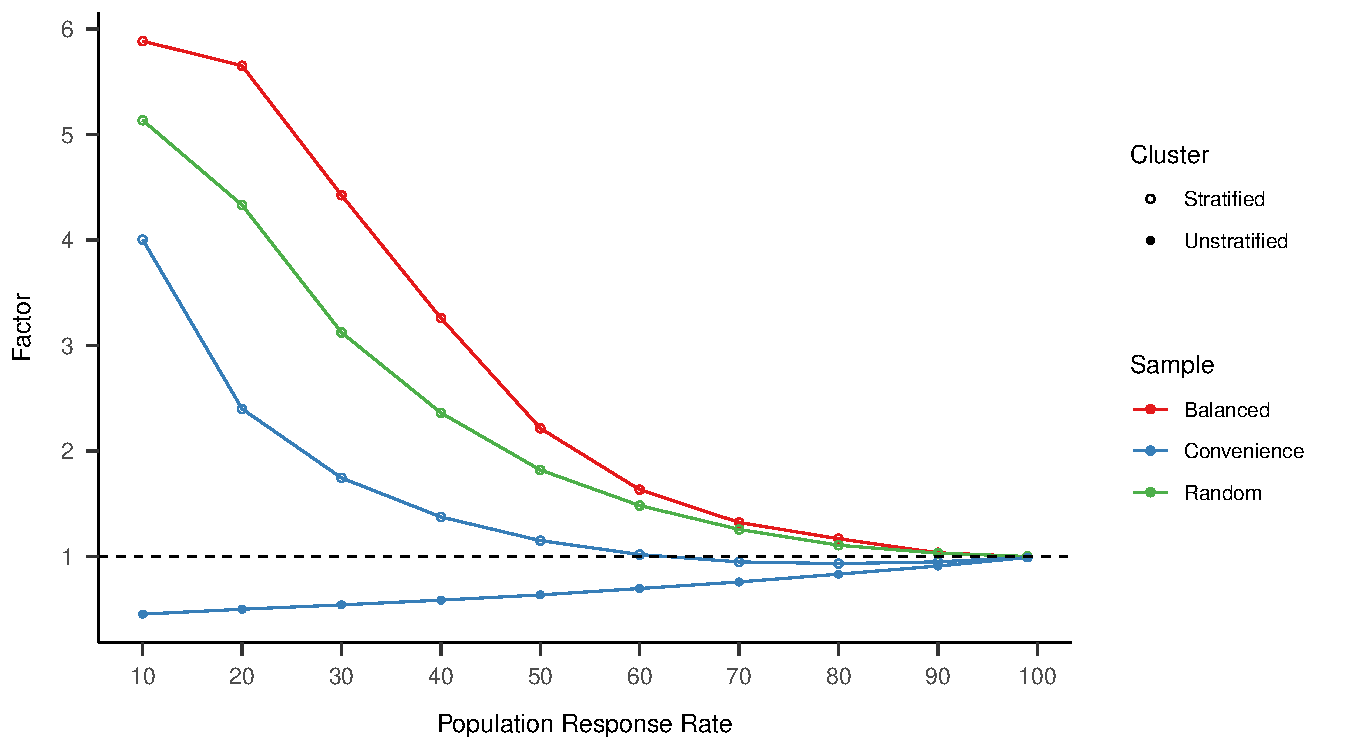
\includegraphics{6---Paper_files/figure-latex/fig-rel-per-1.pdf}
\caption{\label{fig:fig-rel-per}Relative sampling difficulty of each method compared to other methods. The straight horizontal line indicates the reference method being compared to.}
\end{figure}

\hypertarget{sampling-inequality}{%
\subsubsection{Sampling Inequality}\label{sampling-inequality}}

Figure \ref{fig:fig-gini-curve} displays the Gini curve and coefficient for all sampling methods across participation rates. The index is calculated by computing the area between the diagonal line and the curve. Coefficients of 0 indicate uniform equality across all sampling units, i.e.~all schools have an equal opportunity to be sampled. Coefficients of 1 indicate complete inequality, i.e.~very few schools are constantly being sampled across iterations. Overall, stratification results in lower inequality. However, since balanced sampling prioritizes schools according to set characteristics, the same schools are likely to be sampled each time.\todo[color=blue!20]{Again, need to reference the figure in the main text or remove if not needed.}



\begin{sidewaysfigure}[p]
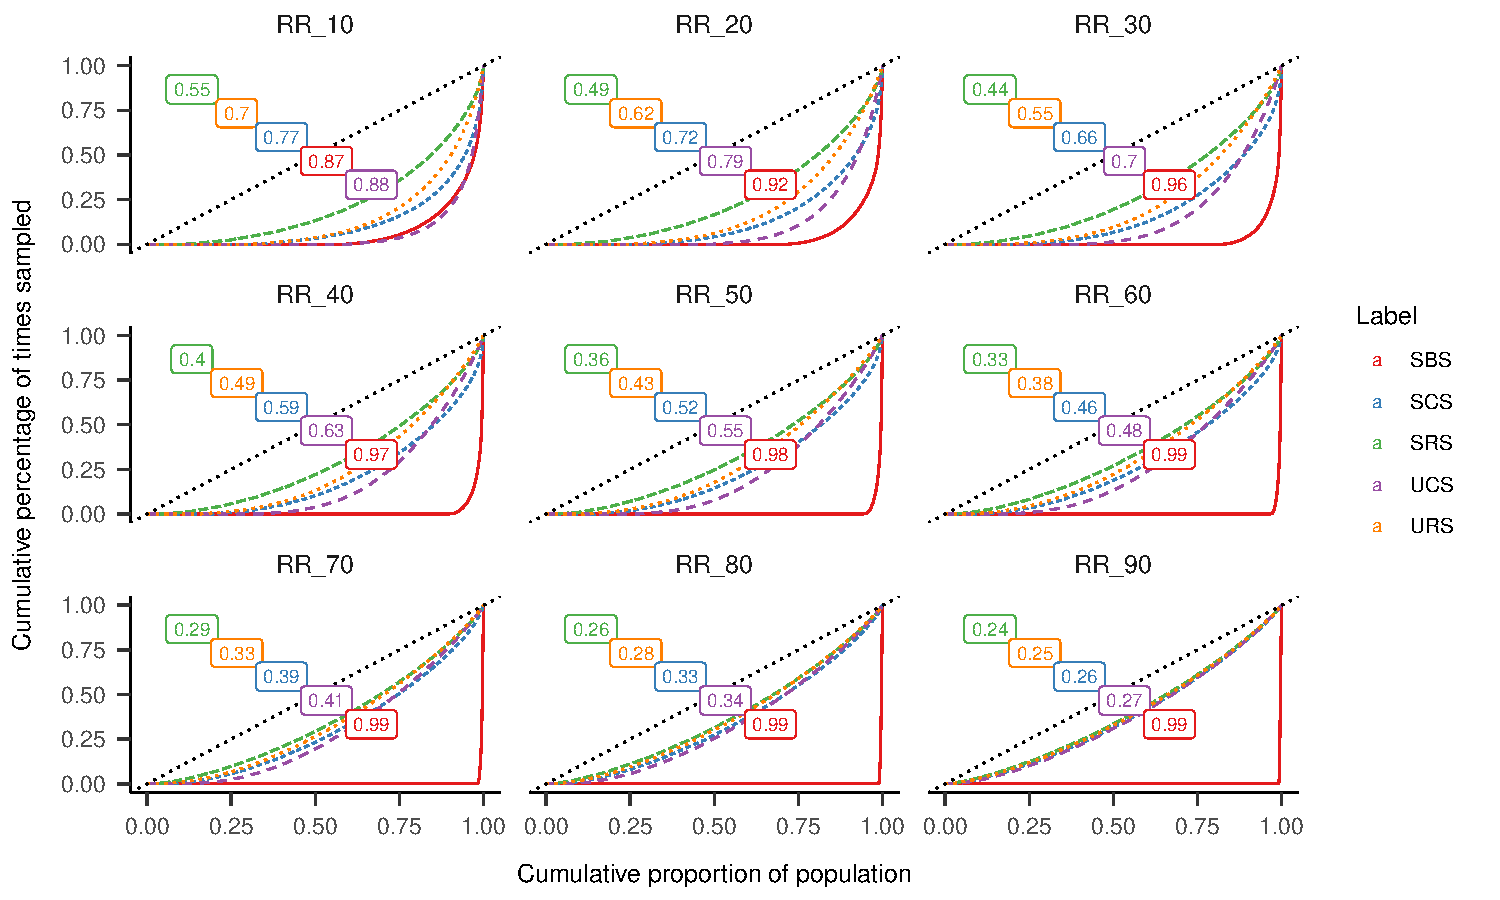
\includegraphics{6---Paper_files/figure-latex/fig-gini-curve-1} \caption{Cumulative probability plot and Gini coefficients representing the inequality of school sampling across sampling methods and population response rates.}\label{fig:fig-gini-curve}
\end{sidewaysfigure}


\end{document}
